%%
%%  chapter07.tex - Obstacle Detection and Planning for Autonomous Vehicles based on Computer Vision Techniques
%%
%%  Copyright 2014 Néstor Morales <nestor@isaatc.ull.es>
%%
%%  This work is licensed under a Creative Commons Attribution 4.0 International License.
%%

\graphicspath{{./images/chapter07/bmps/}{./images/chapter07/vects/}{./images/chapter07/}}

\chapter{Local Planning}\label{ch:chapter07}

Path planning allows an autonomous vehicle to determine the behavior of a vehicle by itself. With this in mind, the vehicle is at this moment able to detect the obstacles in the surrounding area, and has the knowledge of how to reach a certain point in the map from the current position. It is time to make the vehicle drive by itself along this path, avoiding the obstacles in the way.
Despite the global path tell us the safest and shortest path to the goal, we can not use it to directly compute the commands the vehicle needs to start driving, as this global path does not model the long term unpredictability of the environment. Due to the presence of obstacles, this environment is constantly changing. So we need to follow the trajectory using an intermediate mechanism that introduces this short-term information.

\section{The Method}\label{ch:chapter07_01}

The way in which we have solved this problem is based on the method described in \cite{chu2012local} and by \cite{thrun2006stanley}, and modified in order to adapt it to the requirements of our system and the specific characteristics of our prototype, Verdino. Other changes are introduced with the aim of improving the behavior of the whole system.
In our method, we consider the global path obtained in section \todoref{XXX} as the base frame of a curvilinear coordinates system, which will be the paths generation space. The directional information of this path is included, in the way that:
\begin{itemize}
 \item The nearest point (where the distance is computed perpendicular to the global path) to the main trajectory will be the origin of the curvilinear coordinates system.
 \item The horizontal axis will be represented by the distance over global path itself, on its own direction.
 \item The vertical axis is represented by the line perpendicular the origin point, in the left sense regarding to the path direction.
\end{itemize}
With this schema, we can compute easily the trajectories in the curvilinear space (maneuvering information is created), which are then transformed to the initial euclidean space, in which the obstacles information is added by assigning costs to each of the paths.

As said, we were inspired from the works of \cite{chu2012local} and \cite{thrun2006stanley}. From \cite{thrun2006stanley}, we adopted the way in which the distance to the center of the path is used as part of the cost function. However, as explained in the previous section, our path calculation is different due to the environments in which Verdino will be working. In their work, they used a Kalman filter based method.
From \cite{chu2012local}, we based our cost function also in the path smoothness and the cost of the collision with the obstacles computed as a function of the distance to them. This cost is computed by blurring the binary map of the obstacles. In our method, we use a exponential function relative to the distance to the obstacles and the footprint of the car.
We also use as cost functions the length and the curvature of the path. These cost functions will be explained in more detail in section \todoref{XXX}. Both approaches use of a base frame relative to the global path as tool for an easy and efficient computation of the paths.

The obtained algorithm has been applied over Verdino. At the end of this chapter, some experimental results are shown. \comment{Si da tiempo: }Also, there are a set of videos showing the proper behavior of the vehicle in real situations.

The path generation method can be divided in five stages, shown at figure \ref{fig:cp07_pipeline}.
\begin{enumerate}
 \item \emph{Generation of the costmap.} Using the information generated by the sensors, the system constructs a costmap in which costs are related to the distance to the obstacles.
 \item \emph{Base frame construction.} Based on the global path constructed in the previous section (see \todoref{XXX}), we construct the base frame of the curvilinear coordinate system.
 \item \emph{Candidate paths generation.} Candidate paths are generated into the curvilinear space. Then, they are transformed to the euclidean space.
 \item \emph{Selection of the winner path.} Costs of all the paths are assigned, and the one with the lowest value is selected.
 \item \emph{Computation of the vehicle commands.} Vehicle speed and steering angles are computed based on the characteristics of the winner path.
\end{enumerate}

\begin{figure*}[h!]
        \centering
        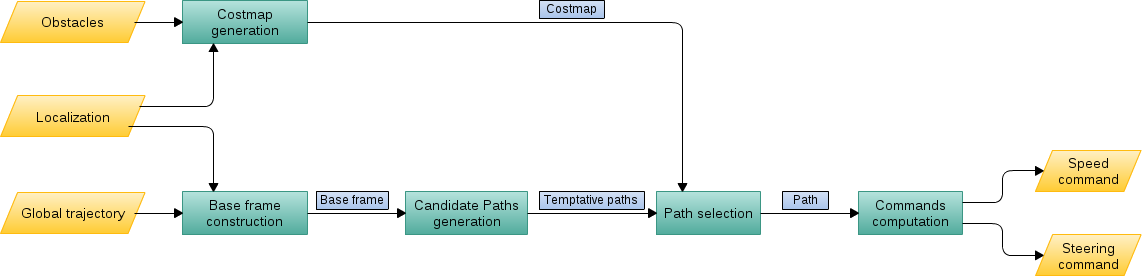
\includegraphics[width=\textwidth]{pipeline}
        \caption{Pipeline of the method described on this chapter.}\label{fig:cp07_pipeline}
\end{figure*}

\subsection{Generation of the costmap}\label{ch:chapter07_01_01}

The costmap maintains information about where the vehicle should navigate in the form of a occupancy grid. It uses sensor data and information from the static map to store and update information about obstacles in the world. In the tests shown in this chapter, information is obtained through the \acp{LIDAR} described at section \todoref{XXX-verdino}. \notsure{Some tests including the information obtained from the methods described in previous sections will be shown at section \todoref{XXX-alltogether}}. Each sensor is used to mark obstacles in the map, or clear them if they are no longer available.

Each cell in the map can have $255$ different cost values:
\begin{itemize}
 \item A value of $255$ means that we do not have information about an specific cell in the map.
 \item $254$ means that a sensor has marked this specific cell as occupied, which is considered as a lethal cell. The vehicle should never enter into this cell.
 \item The rest of cells are considered as free, but with different cost levels depending on an inflation method relative to the size of the vehicle and its distance to the obstacle.
\end{itemize}

Cost values out from occupied cells decrease with distance using the following expression:

\begin{equation}\label{eq:cp07_costmap_inflation}
 \mathcal{C}(i, j) = \exp (-1.0 \cdot \alpha \cdot ( \|c_{ij}-\vec{o}\| - \rho_{inscribed})) \cdot 253
\end{equation}

In this expression, $\alpha$ is a scaling factor that allows increasing or decreasing the decay rate of the cost of the obstacle. $\|c_{ij}-\vec{o}\|$ is the distance between the cell $c_{ij} \in \mathcal{C}$ (where $\mathcal{C}$ is the set of cells in the costmap) and the obstacle. Finally, $\rho_{inscribed}$ is the inscribed radius, which is the inner circle of the limits of the car. This radius is depicted in the figure \ref{fig:cp07_costmap_concepts}.

\begin{figure}[h!]
\begin{tabular}{cc}
  \begin{subfigure}[b]{0.5\textwidth}
    \centering
    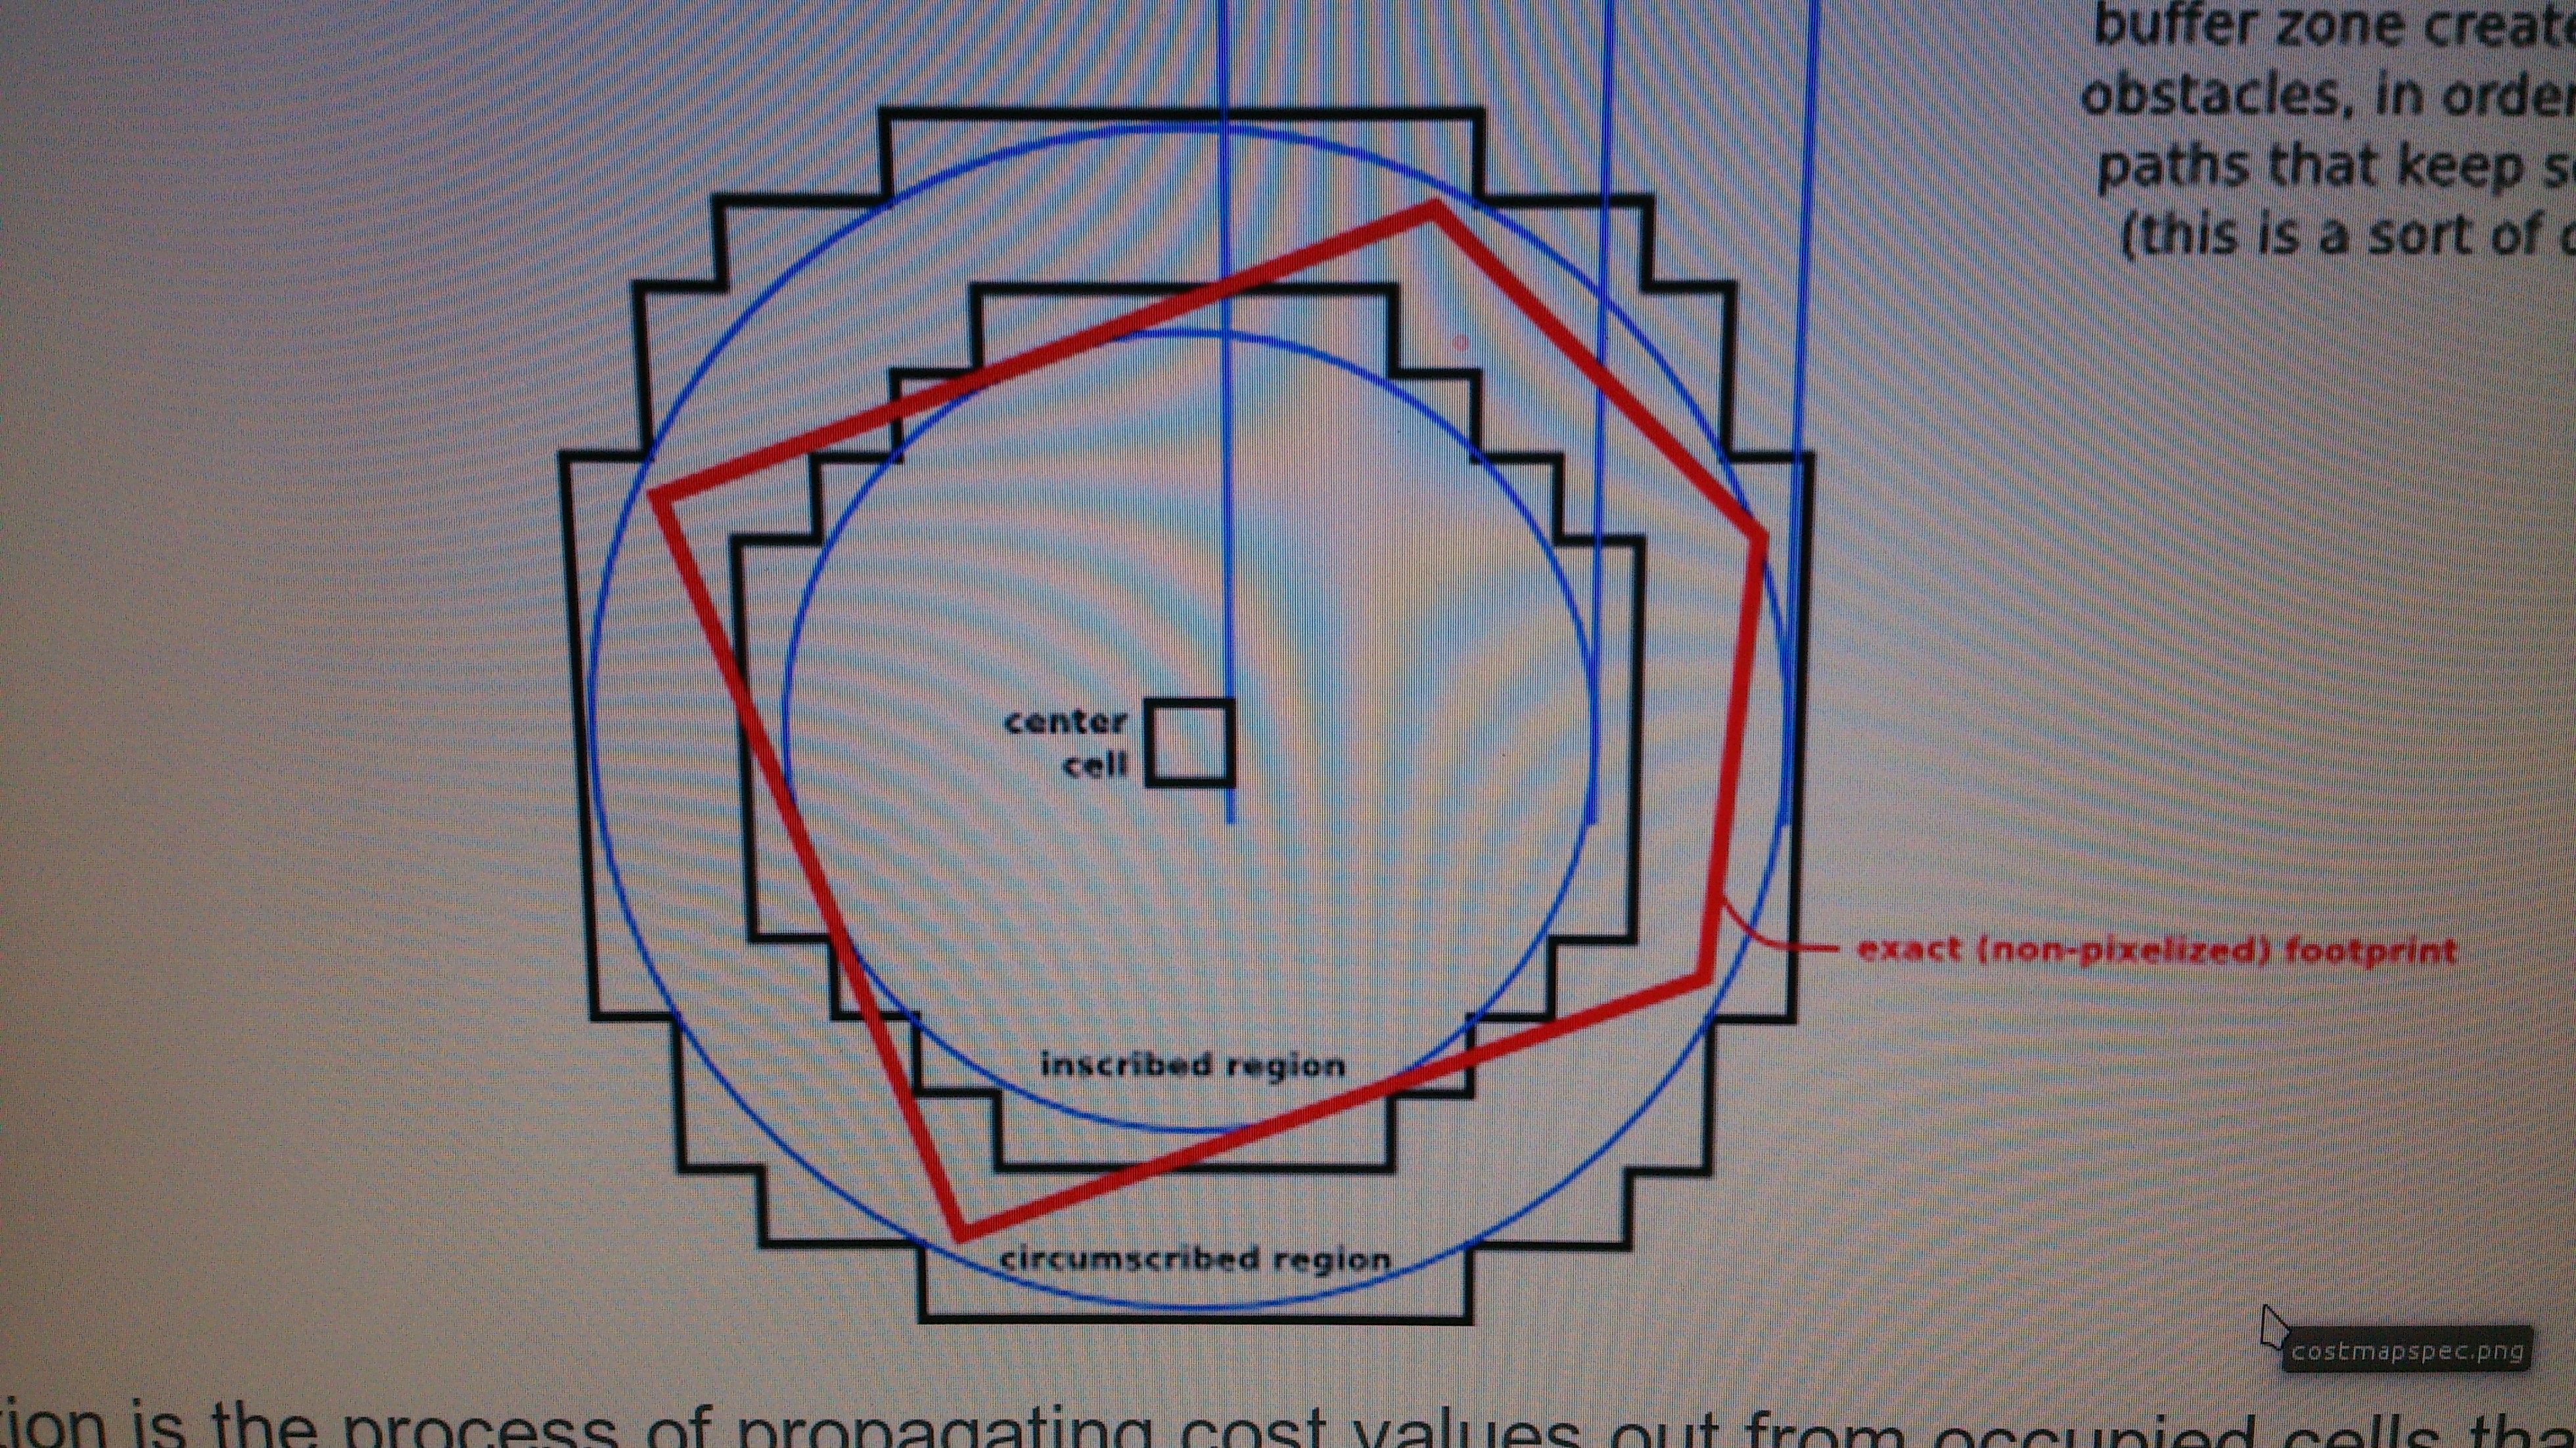
\includegraphics[width=\textwidth, trim=50 40 80 60,clip]{inscribed_circumscribed}
    \caption{$\tau_{inscribed}$ and $\tau_{circumscribed}$.}
    \label{fig:cp07_inscribed_circumscribed}
  \end{subfigure} &
  \begin{subfigure}[b]{0.5\textwidth}
    \centering
    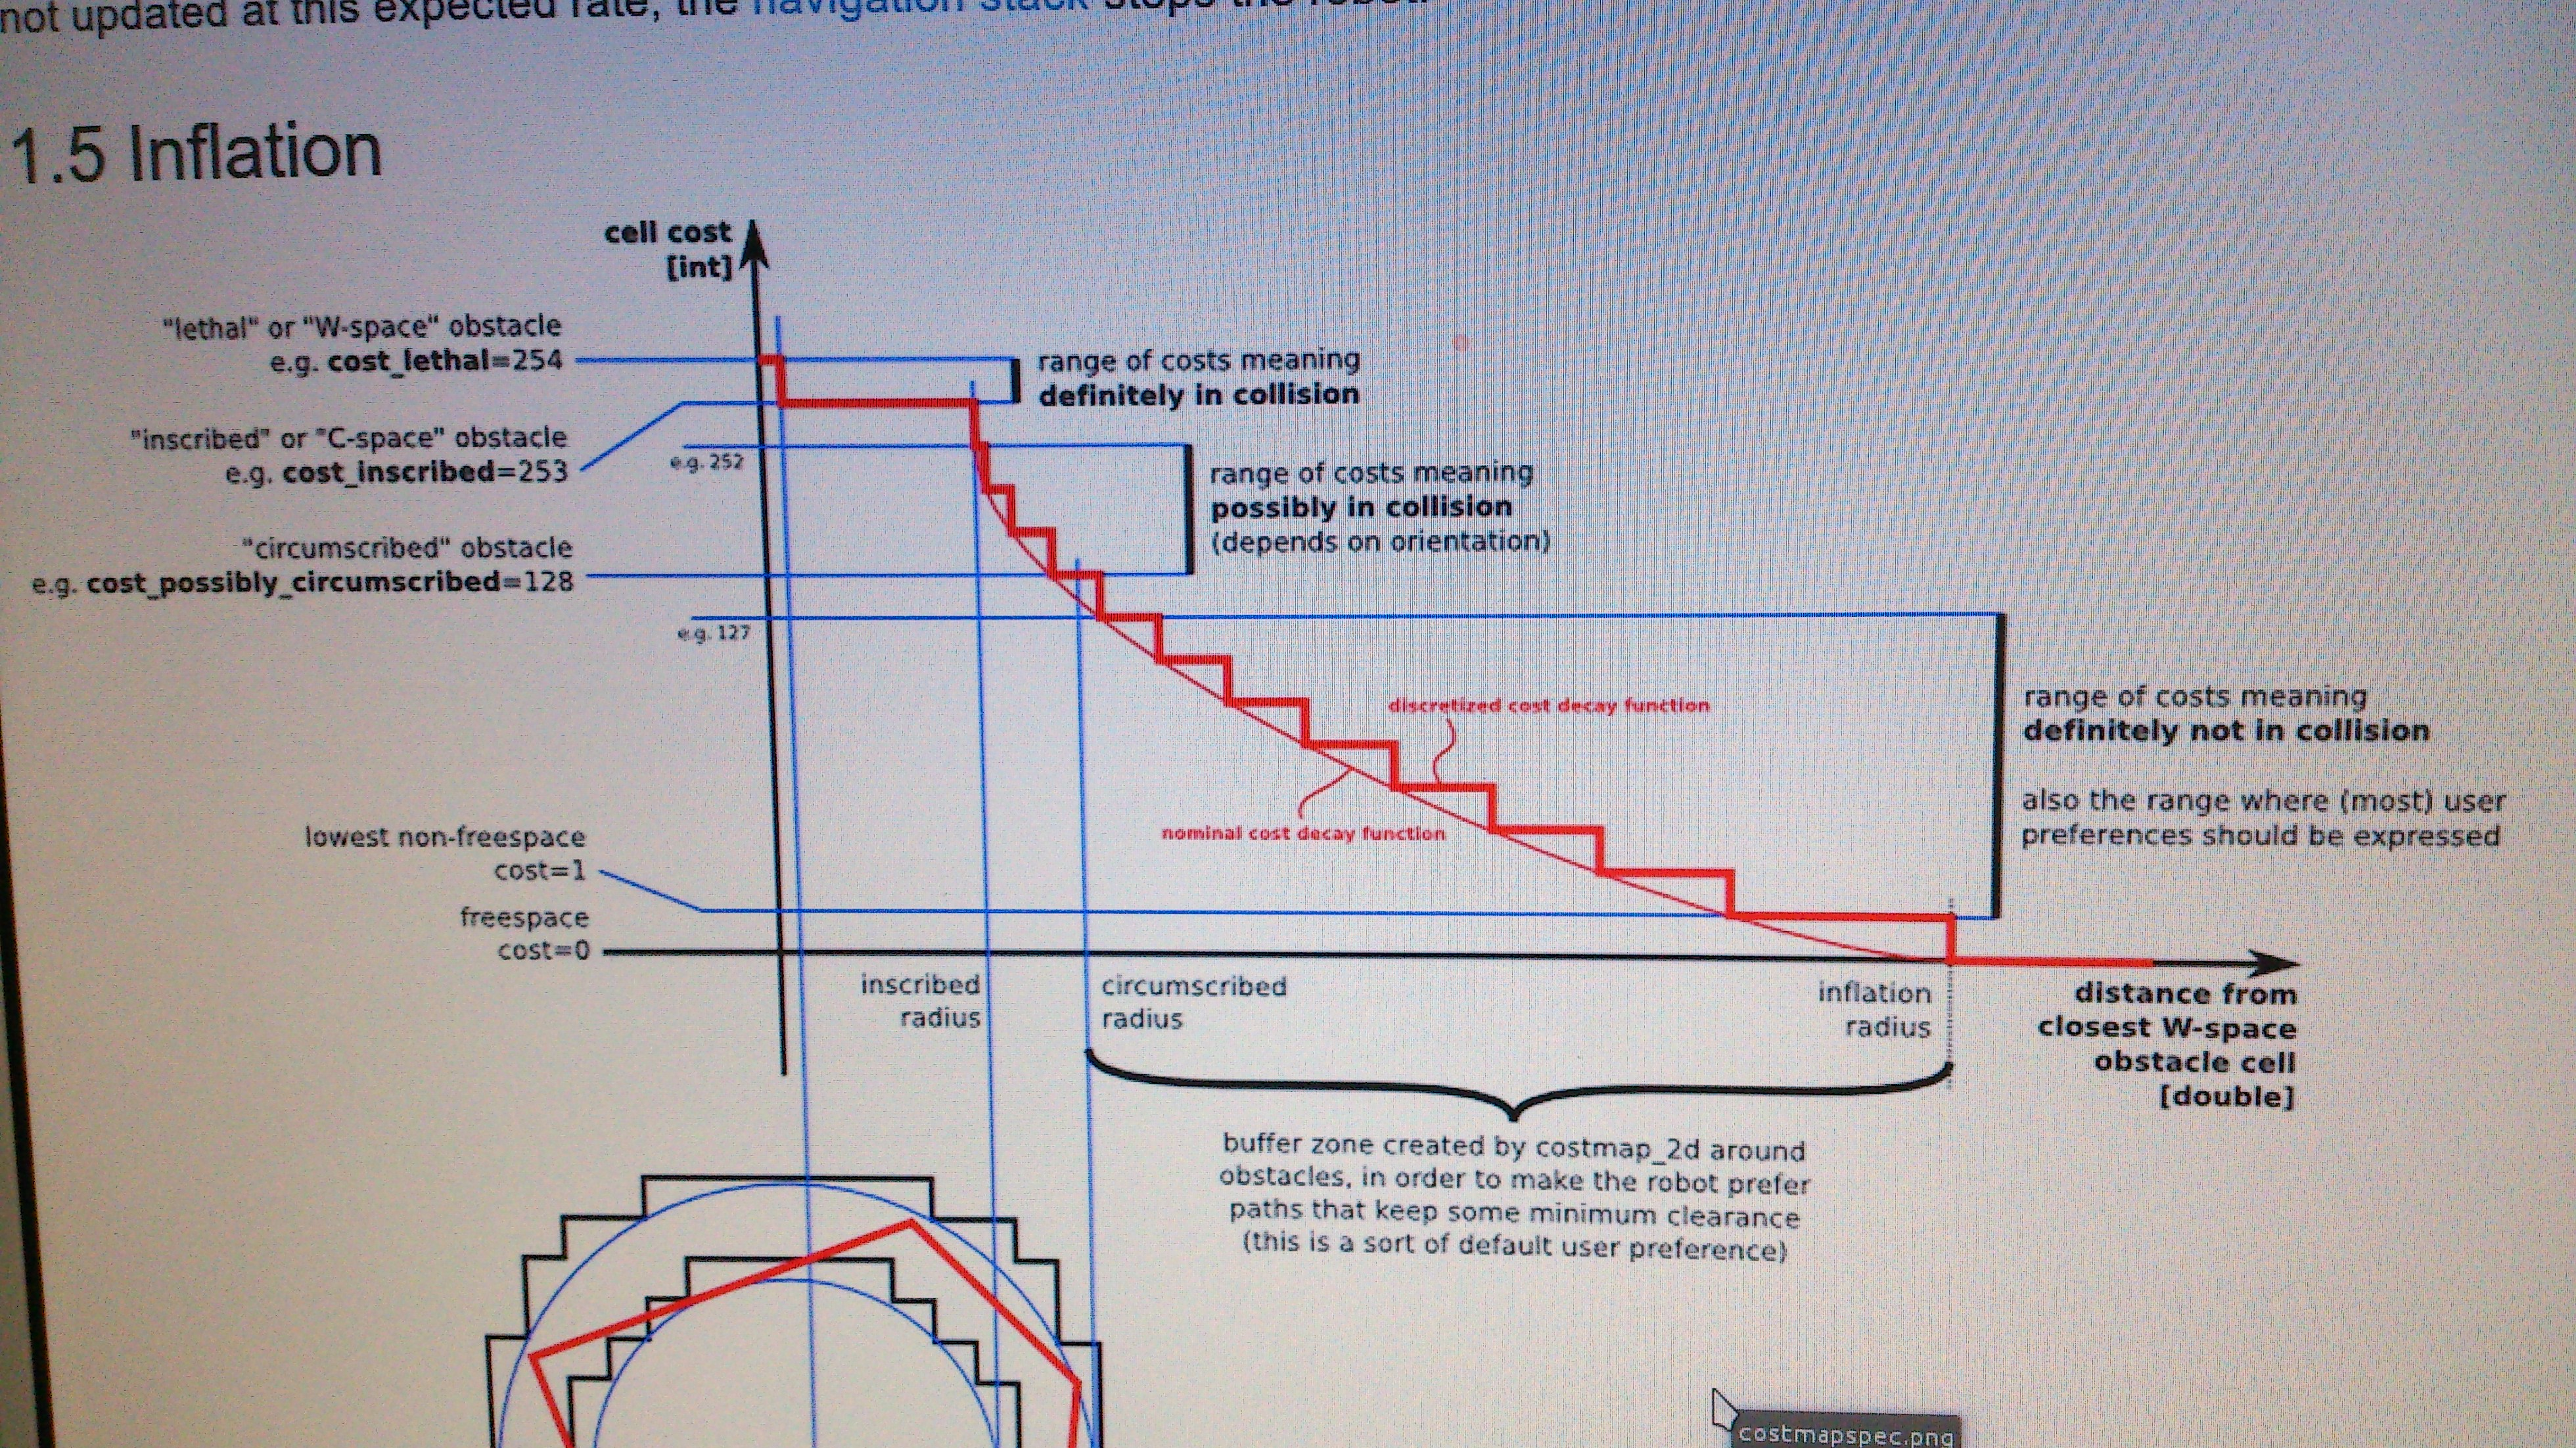
\includegraphics[width=\textwidth, trim=50 40 80 60,clip]{cost_levels}
    \caption{Cost levels.}
    \label{fig:cp07_cost_levels}
  \end{subfigure}% 
\end{tabular}
\caption{Costmap computation concepts.}\label{fig:cp07_costmap_concepts}
\end{figure}

Despite all of them are free cells, we define four different distance thresholds in order to set different danger levels in the map, depicted in figure \ref{fig:cp07_costmap_concepts}:

\begin{itemize}
 \item $\tau_{lethal}$: There is a obstacle in this cell, marked by the sensor. Corresponds to the cost level $254$. The vehicle is in collision.
 \item $\tau_{inscribed}$: The cell distance to the nearest obstacle is below the value $\rho_{inscribed}$. If the center of the vehicle is in this cell, it is also in collision, so the areas below this distance threshold should be avoided. The cost level is always $253$.
 \item $\tau_{circumscribed}$: If the vehicle center is on this cell, there are chances to be in collision with an obstacle, depending on its orientation. A cell with a distance to an obstacle below this threshold should be avoided, but there are possibilities to be in one of them without colliding an obstacle. The rest of cells are assumed to be safe (except from those with \emph{unknown} cost).
\end{itemize}

We just consider in our approach the paths passing along areas with a distance to an obstacle over $\tau_{circumscribed}$, for which a cost will be assigned based on the equation \ref{eq:cp07_costmap_inflation} and other cost factors that will be explained later. Paths passing trough the rest of cells will be truncated at the last safe point.

For optimization reasons, we do not compute the costmap of the whole map at each iteration. Instead, we just compute the cells in a $40x40\,m$ area centered into the current car position. 

In the development of this method, we used the \ROS plugin \program{costmap\_2d}\footnote{\url{http://wiki.ros.org/costmap\_2d}}, which implements the functionalities described in this section. 

\subsection{Base frame construction}\label{ch:chapter07_01_02}

Instead of locating the vehicle in the new created frame, as done in \cite{chu2012local}, at each iteration we prune the global plan up to its nearest point to the car location, so the origin of the base frame will be the first point in the pruned global plan. This distance is measured in terms of the euclidean distance in the direction perpendicular to each point in the path. If the pruned plan is valid and its size is different from zero, we start the base frame construction stage.

In this stage, we will define the base frame of the curvilinear coordinate system, so the algorithm will be able to compute the trajectories in this space as if the global plan were a rectilinear trajectory. The geometric relationship between the path in euclidean coordinates and curvilinear coordinates is shown at figure \ref{fig:cp07_euclidean_frenet_conversion}.

\begin{figure}[h!]
\begin{tabular}{cc}
  \begin{subfigure}[b]{0.5\textwidth}
      \centering
      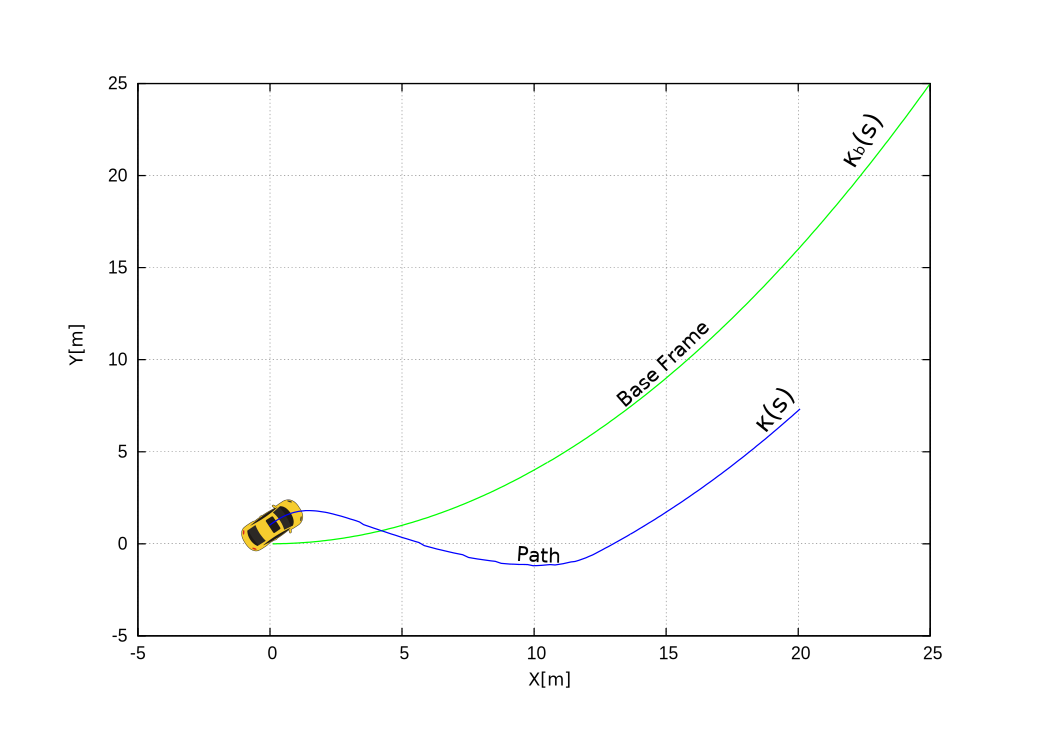
\includegraphics[width=\textwidth, trim=50 40 80 60,clip]{justOneCartesian45}
      \caption{Euclidean space.}
      \label{fig:cp07_justOneCartesian45}
  \end{subfigure} &
  \begin{subfigure}[b]{0.5\textwidth}
    \centering
    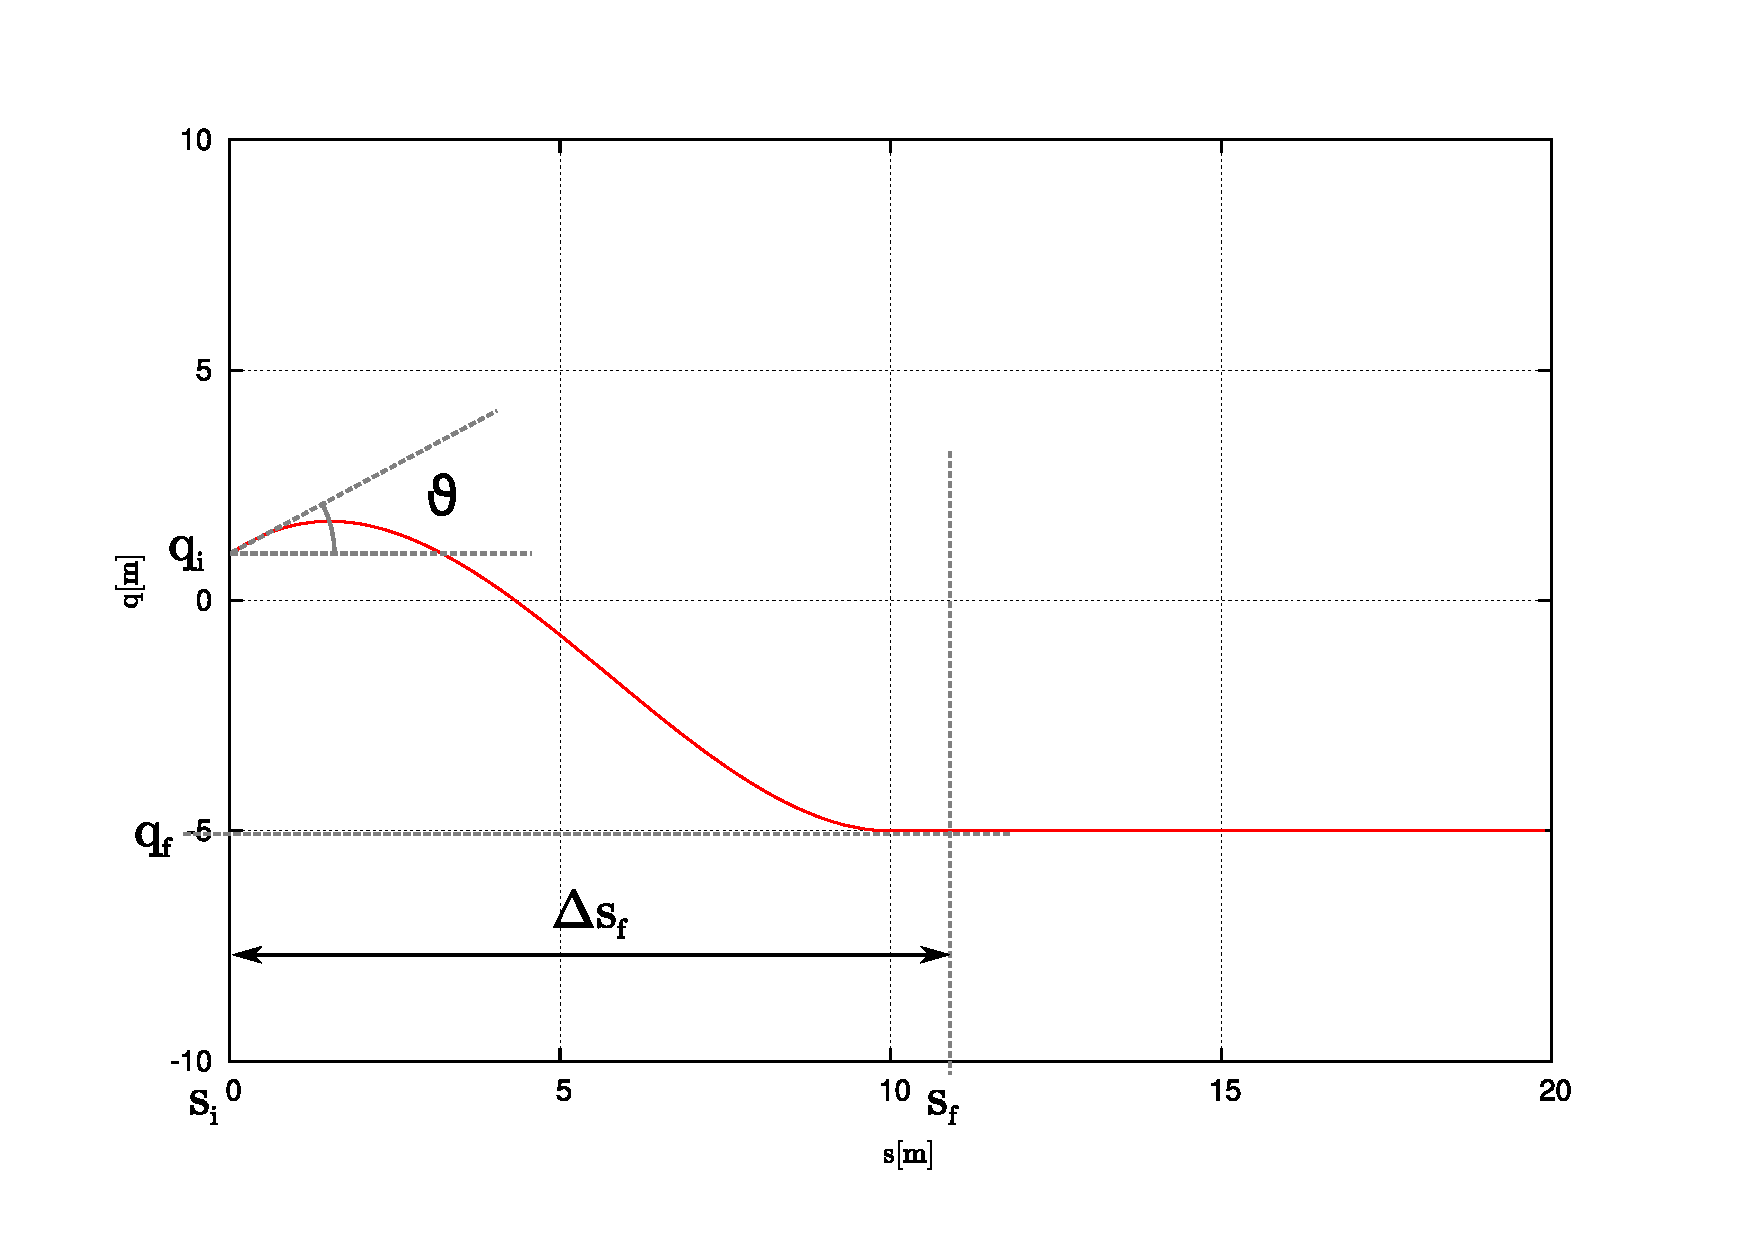
\includegraphics[width=\textwidth, trim=50 40 80 60,clip]{justOneFrenet45}
    \caption{Curvilinear space.}
    \label{fig:cp07_justOneFrenet45}
  \end{subfigure}%   
\end{tabular}
\caption{Conversion of a trajectory between the Cartesian and Frenét spaces. \todo{Incluir la información disponible en el paper original para estas figuras (9 y 10)}}\label{fig:cp07_euclidean_frenet_conversion}
\end{figure}


There, the longitude of the arc of the base frame ($s$, on the right image) is the distance along the global plan, which is represented as a green line. This distance is represented by the horizontal axis of the curvilinear system. The vertical axis, $q$, represents the perpendicular lateral distance respect to the path, so the left side is represented by positive values and the right by the negatives.

For the computation of the transformation between the euclidean coordinate system and the curvilinear, we need to compute the value $\kappa$, which represents the path curvature. This value is computed as follows (\cite{chu2012local}, \cite{werling2010optimal}, \cite{barfoot2004motion})

\begin{equation}\label{eq:cp07_path_curvature}
 \kappa = {S \over Q} \cdot \left ( \kappa_b \cdot { 
 {(1 - q \cdot \kappa_b) \cdot (\partial^2q / \partial s^2) +
 \kappa_b \cdot (\partial q / \partial s )^2
 } 
 \over {Q^2} } \right )
\end{equation}

,where 

\begin{equation}\label{eq:cp07_path_curvature_s_and_q}
\begin{cases}
S=sign(1 - q \cdot \kappa_b)\\
Q=\sqrt{\left ( { {\partial q} \over {\partial s}} \right ) ^2+ (1 - q \cdot \kappa_b)^2}
\end{cases}
\end{equation}

Based on this, each generated path will be rejected in the following cases:
\begin{itemize}
 \item The lateral offset $q$ is similar to the curvature radius of the base frame $1 / \kappa_b$. In this case, the path passes through the center of curvature of the base frame.
 \item $q > {1 \over \kappa_b}$. In this case, the curvature and direction of the generated path has a sign opposed to the direction of the base frame. Path should be discarded, as it violates the non-holonomic condition of the movement of the vehicle.
\end{itemize}

Also, the maximal curvature a path can have in order to be feasible by the vehicle is limited by a restriction in the steering angle. If this restriction is violated, the corresponding path is rejected. This curvature is directly related to the movement of the vehicle, which can be described through several models. A simplified version, which ignores the related physical effects (like inertia or mass), is (\cite{chu2012local}, \cite{barfoot2004motion}):

\begin{equation}\label{eq:cp07_simplified_motion_model}
\begin{cases}
\dot{x} = |\vec{v}| \cdot cos(\theta) \\
\dot{y} = |\vec{v}| \cdot sin(\theta) \\
\dot{\theta} = |\vec{v}| \cdot \kappa
\end{cases}
\end{equation}

As these physical effects does not affect to the geometric shape of the path, we can avoid their usage. In equation \ref{eq:cp07_simplified_motion_model}, $[\dot{x} \dot{y} \dot{\theta} ]^T$ are the estimated position and orientation of the vehicle and $|\vec{v}|$ is the module of the speed. Taking into account this simplified model, we can assume that the vehicle just have two degrees of freedom, corresponding to the speed $\vec{v}$ and $\kappa$. As at this point we are just interested into the geometric generation of the path, we can remove the speed of the vehicle $\vec{v}$ from the model. The way in which this is done is by expressing the movement of the vehicle in terms of the traveled distance. So the following relation is established (\cite{chu2012local}):

\begin{equation}\label{eq:cp07_speed_to_distance}
|\vec{v}| = S \cdot Q \cdot { {\partial s} \over {\partial t}}
\end{equation}

If the speed of the vehicle is substituted into the model described in equation \ref{eq:cp07_simplified_motion_model}, the differential equation of the movement can be represented regarding to the arc length of the base frame as:

\begin{equation}\label{eq:cp07_motion_model_in_distance_terms}
\begin{cases}
{{\partial x} \over {\partial s}} = Q \cdot cos(\theta) \\
{{\partial y} \over {\partial s}} = Q \cdot sin(\theta) \\
{{\partial \theta} \over {\partial s}} = Q \cdot \kappa
\end{cases}
\end{equation}

The advantages of this new model is that it can be generated independently from the vehicle speed along the base frame.

\subsection{Candidate paths generation}\label{ch:chapter07_01_03}

As said previously, the generation of the paths corresponding to each of the maneuvers the car can follow is performed in the curvilinear space, independently from the obstacles in the environment. These will be taken into account later, once the tentative trajectories have been transformed to the euclidean space.

\subsubsection{Maneuvering paths generation}\label{ch:chapter07_01_03_01}

In order to generate a path, its curvature is defined by the lateral offset $q$ respect to the base frame. First and second order derivatives of $q$ are needed if we want to compute $\kappa$ (see equations \ref{eq:cp07_path_curvature} and \ref{eq:cp07_path_curvature_s_and_q}), so we need a function dependent to the lateral offset if we want a smooth lateral change.

$q$ can be defined by a sequence of a cubic polynomial and a set of constants:

\begin{equation}\label{eq:cp07_function_q}
\begin{align*}
q(s) &=
  \begin{cases}
   a \cdot \Delta s^3 + b \cdot \Delta s^2 + c \cdot \Delta s + q_i & \text{if } s_i \le s < s_f \\
   q_f        & \text{if } s_f \le s
  \end{cases}\\
{{\partial q} \over {\partial s}}(s) &=
  \begin{cases}
   3 \cdot a \cdot \Delta s^2 + 2 \cdot b \cdot \Delta s + c & ~~~~~~~\text{if } s_i \le s < s_f \\
   0        & ~~~~~~~\text{if } s_f \le s
  \end{cases}\\
{{\partial^2 q} \over {\partial s^2}}(s) &=
  \begin{cases}
   6 \cdot a \cdot \Delta s + 2 \cdot b & ~~~~~~~~~~~~~~~~~~~~~~~\text{if } s_i \le s < s_f \\
   0        & ~~~~~~~~~~~~~~~~~~~~~~~\text{if } s_f \le s
  \end{cases}
\end{align*}
\end{equation}

, where $\Delta s = s - s_i$.

In figure \ref{fig:cp07_euclidean_frenet_conversion}, the components involved in this process are depicted.
\begin{itemize}
 \item The initial lenght $s_i$ is zero, due to the prune task performed to the path at the beginning of each iteration. Lateral offset $q_i$ is also known, which is the lateral offset to the initial point of the global path.
 \item Angle $\theta$ defines the difference between the vehicle heading angle and the tangent angle of the base frame.
 \item $s_f$ is a parameter that allows controlling the longitudinal distance needed to reach the offset $q_f$. This distance should be dependent from the speed. However, as the maximal speed of the prototype is not too hight, we can set $\Delta s_f$ as the distance needed to go from $q_i$ to the biggest $q_f$ at the maximal speed.
 \item $q_f$s are computed for each path attending to the parameters defined by the user. $s_f$ is also a parameter.
\end{itemize}

Parameters $s_i$, $q_i$, and $s_f$ are the same for all the candidate paths. By modifying the value of $q_f$ we get the different paths. To do that, we divide the width of the road into as many segments as the desired number of paths. Then, $q_f$ will be a distance, perpendicular to the base frame, between the global path and the corresponding road width division depending on the number of path being generated. Using this technique, the desired number of paths is created, each of them with a different lateral offset $q_f$. The set of paths should cover the whole road width, so the vehicle should be able to avoid the obstacles if possible.

In our tests, we have considered a maximal width of 4\,m (a little bit above the width of the roads in our testing area), with an horizon of 10\,m in the direction of the global path. This horizon gives us a prediction of 2\,seconds at the maximal speed of the vehicle. We evaluate a total of 21 paths, with a distance between them ($\Delta q_f$) of 20\,cm.

\subsubsection{Candidate paths generation}\label{ch:chapter07_01_03_02}

Once we have computed the paths in the curvilinear coordinate system, we transform them so we they can be used in the euclidean space. In this new space, we will be able to evaluate their associated costs, as those related to the distance to obstacles, smoothness, etc. In figures \ref{fig:cp07_frenet0} and \ref{fig:cp07_frenet45}, we can see two examples of this process.

In figure \ref{fig:cp07_frenet0}, an example in which the vehicle is at a lateral distance of 1\,m respect to the base frame, and the orientation of the vehicle regarding to this base frame is 0. That is, $q_i = 1$, $s_i = 0$ and $\theta = 0$. In the left image, we see that the set of paths is symmetric, being the central path completely parallel to the axis $s$. These trajectories are then projected to the euclidean space, obtaining the paths represented in the right image. There, the green line represents the global path, and the blue lines are the projected candidate paths. As can be seen, they fit properly to the global path.

\begin{figure}[h!]
\begin{tabular}{cc}
  \begin{subfigure}[b]{0.5\textwidth}
    \centering
    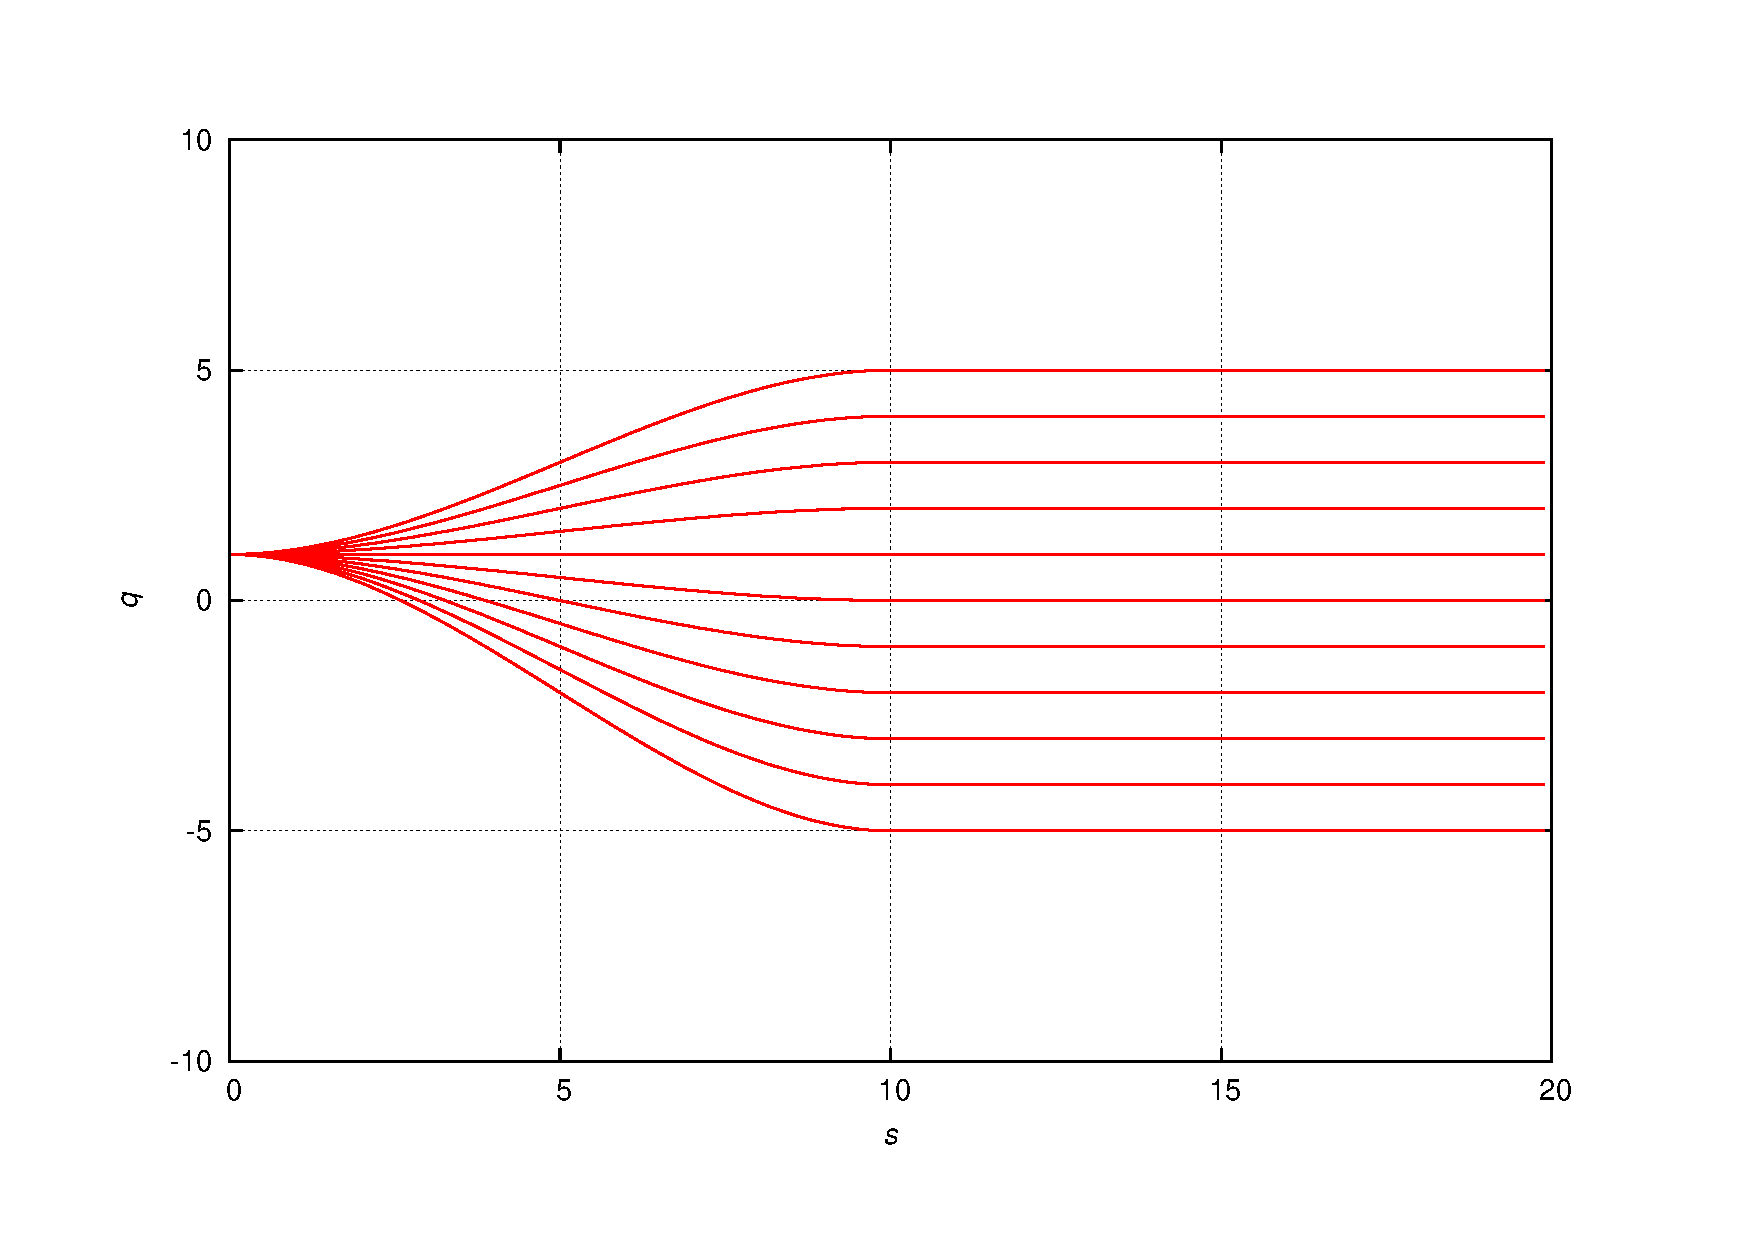
\includegraphics[width=\textwidth, trim=50 40 80 60,clip]{frenet0}
    \caption{Curvilinear space.}
    \label{fig:cp07_frenet0}
  \end{subfigure} &
  \begin{subfigure}[b]{0.5\textwidth}
    \centering
    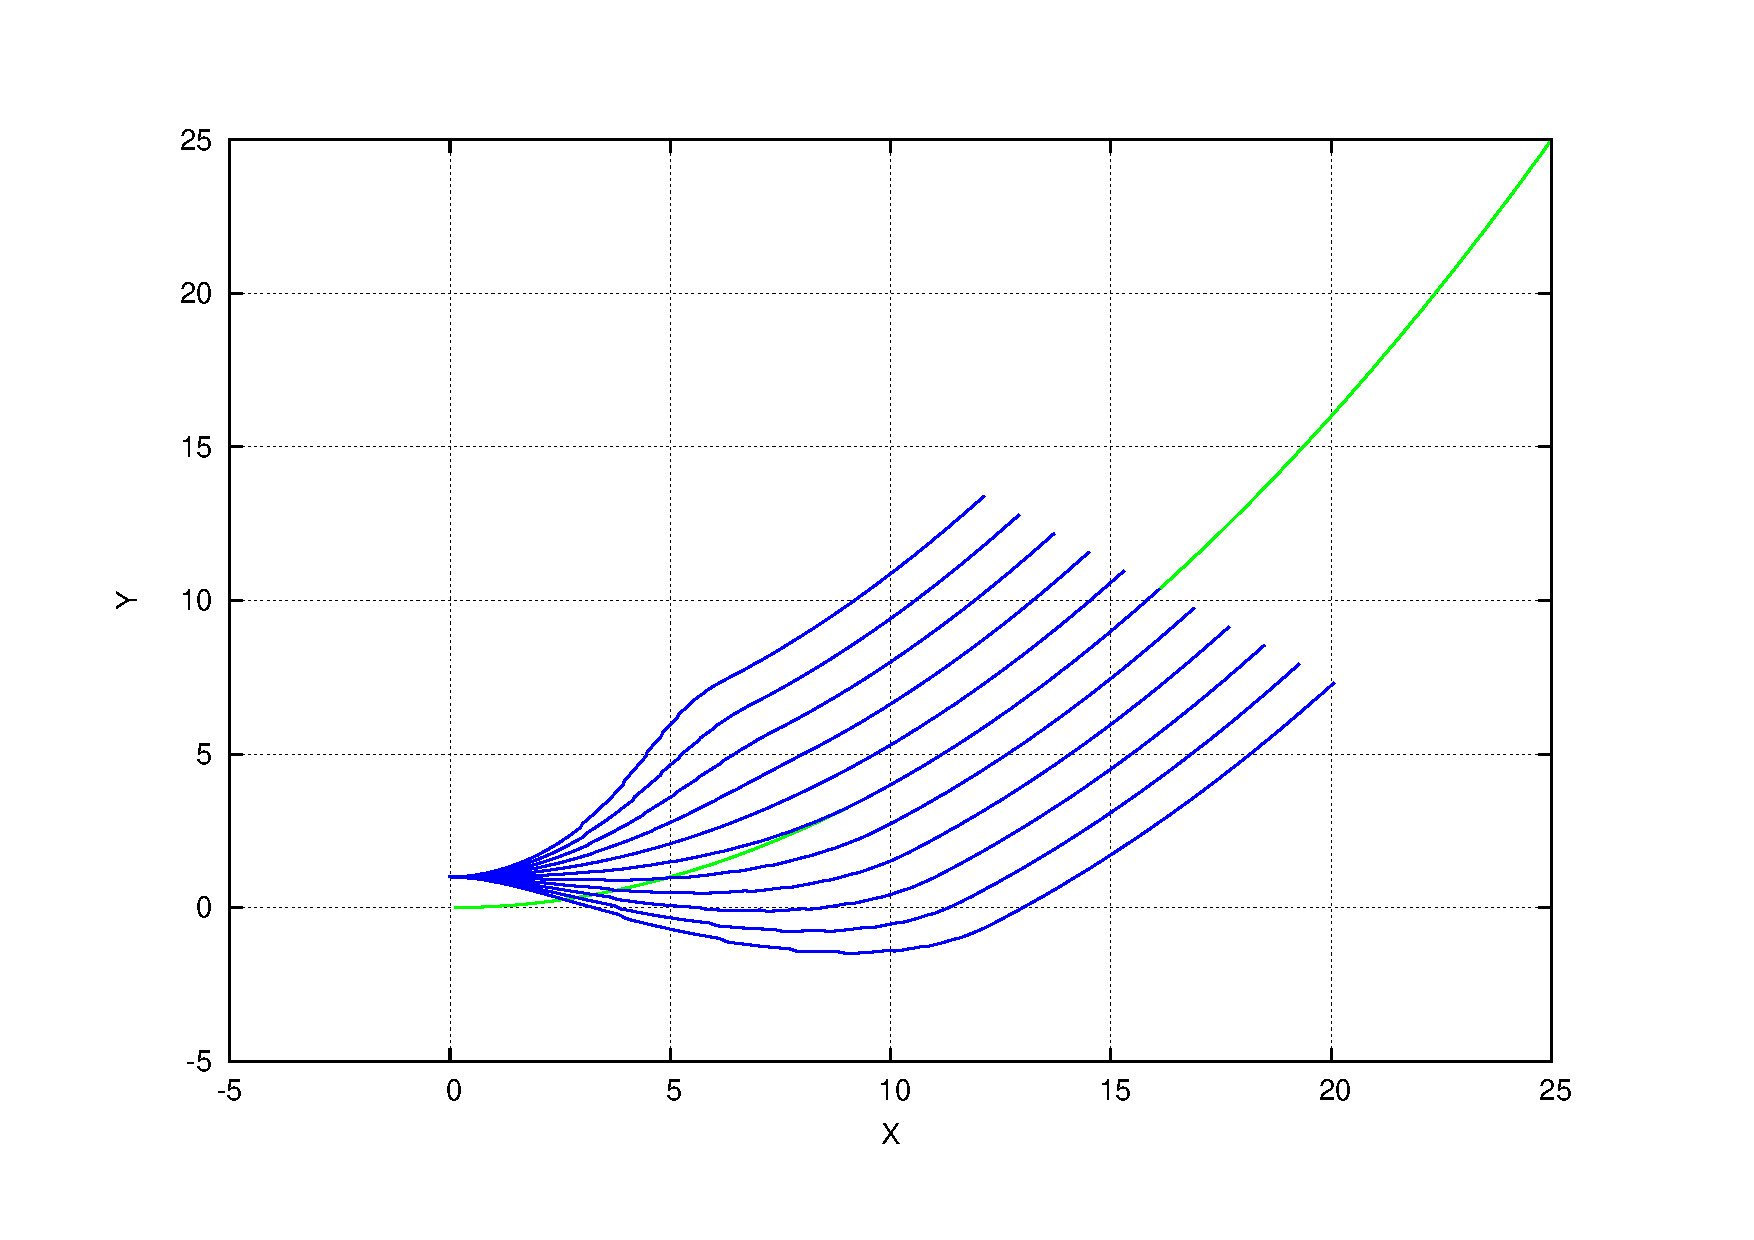
\includegraphics[width=\textwidth, trim=50 40 80 60,clip]{cartesian0}
    \caption{Curvilinear space.}
    \label{fig:cp07_cartesian0}
  \end{subfigure}%
\end{tabular}
\caption{Example in which the vehicle is oriented parallel to the path.}\label{fig:cp07_frenet0}
\end{figure}

In figure \ref{fig:cp07_frenet45}, a similar example is shown. The only difference is that, this time, the vehicle is oriented $45^\circ$ away from the base frame orientation. This causes the paths in the curvilinear space to move away from the $s$ axis until they start converging. Same effect occurs in the transformed euclidean paths: they get away from the global path but, after a few meters, they start approaching to it.

\begin{figure}[h!]
\begin{tabular}{cc}
  \begin{subfigure}[b]{0.5\textwidth}
    \centering
    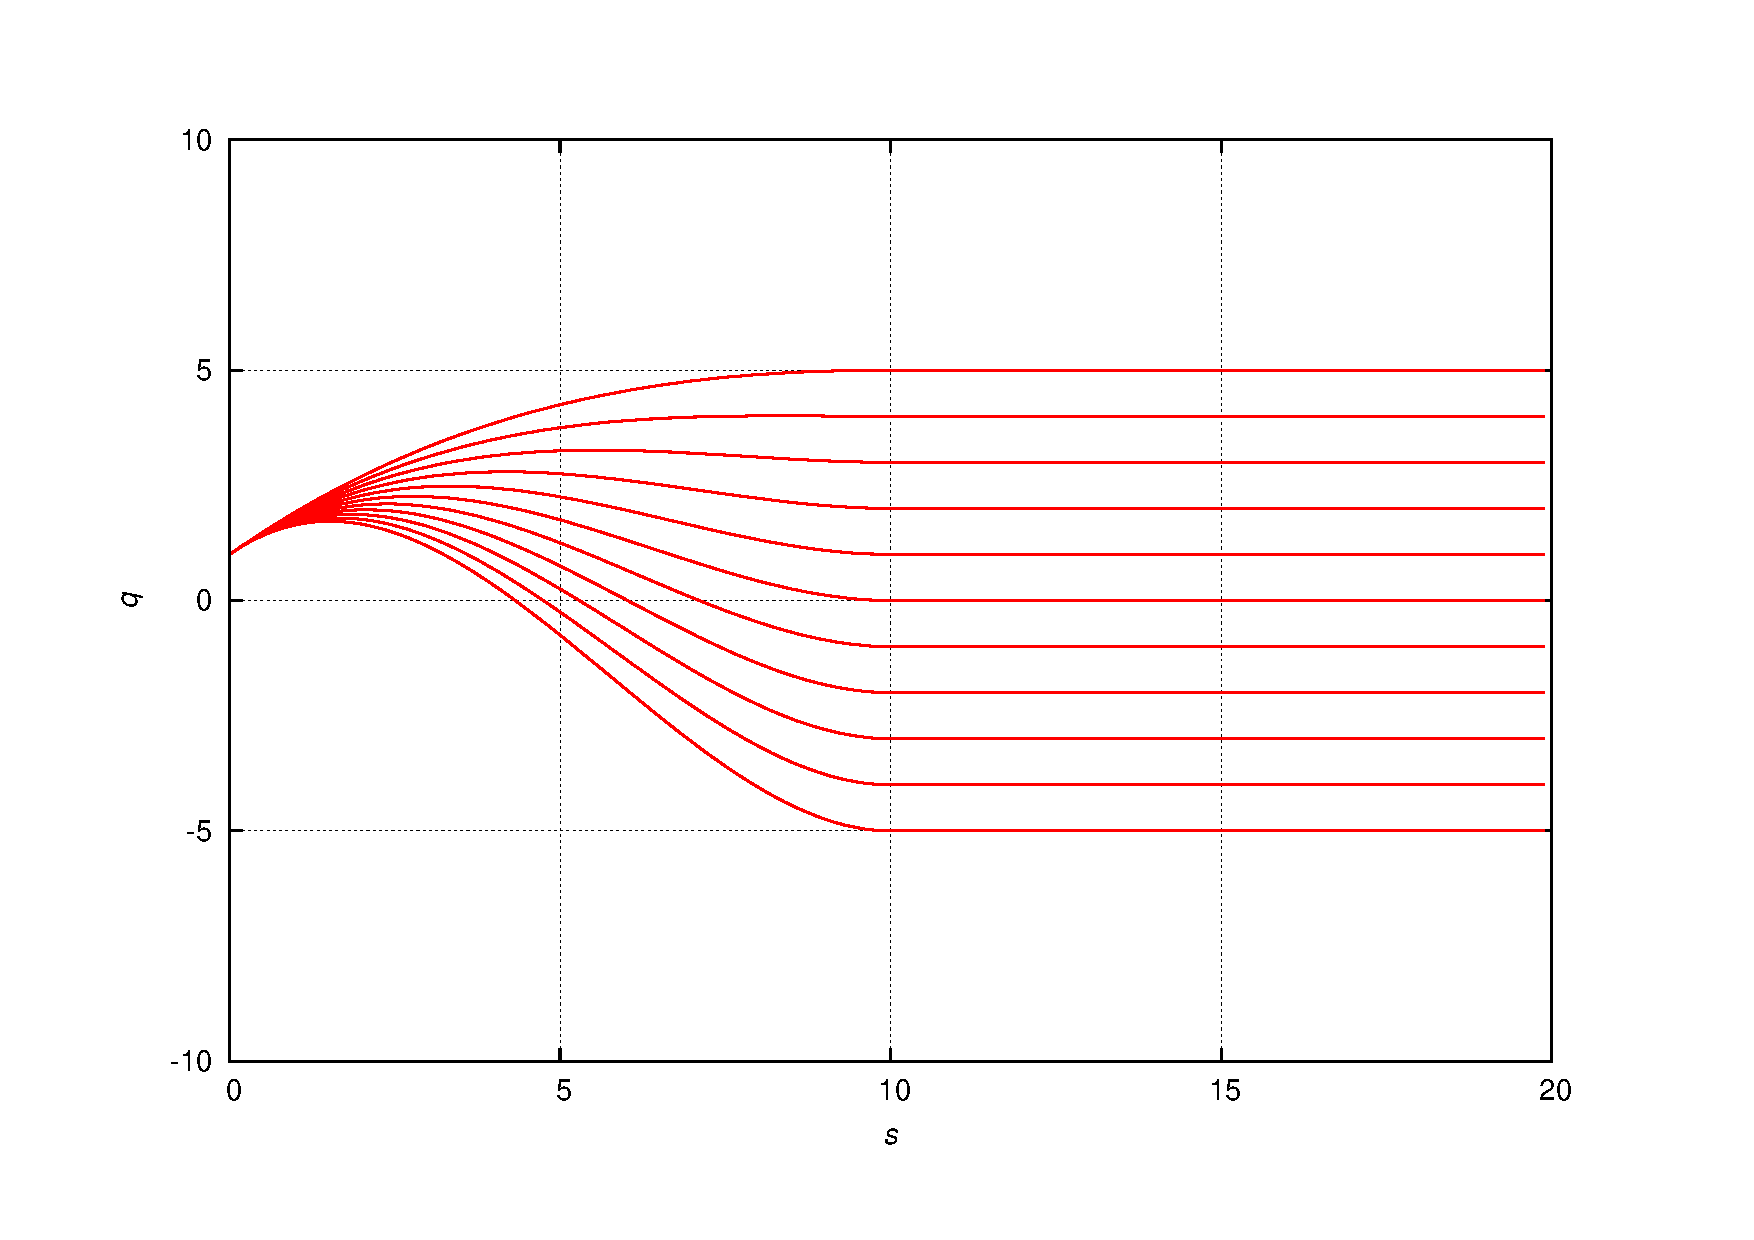
\includegraphics[width=\textwidth, trim=50 40 80 60,clip]{frenet45}
    \caption{Curvilinear space.}
    \label{fig:cp07_frenet45}
  \end{subfigure} &
  \begin{subfigure}[b]{0.5\textwidth}
    \centering
    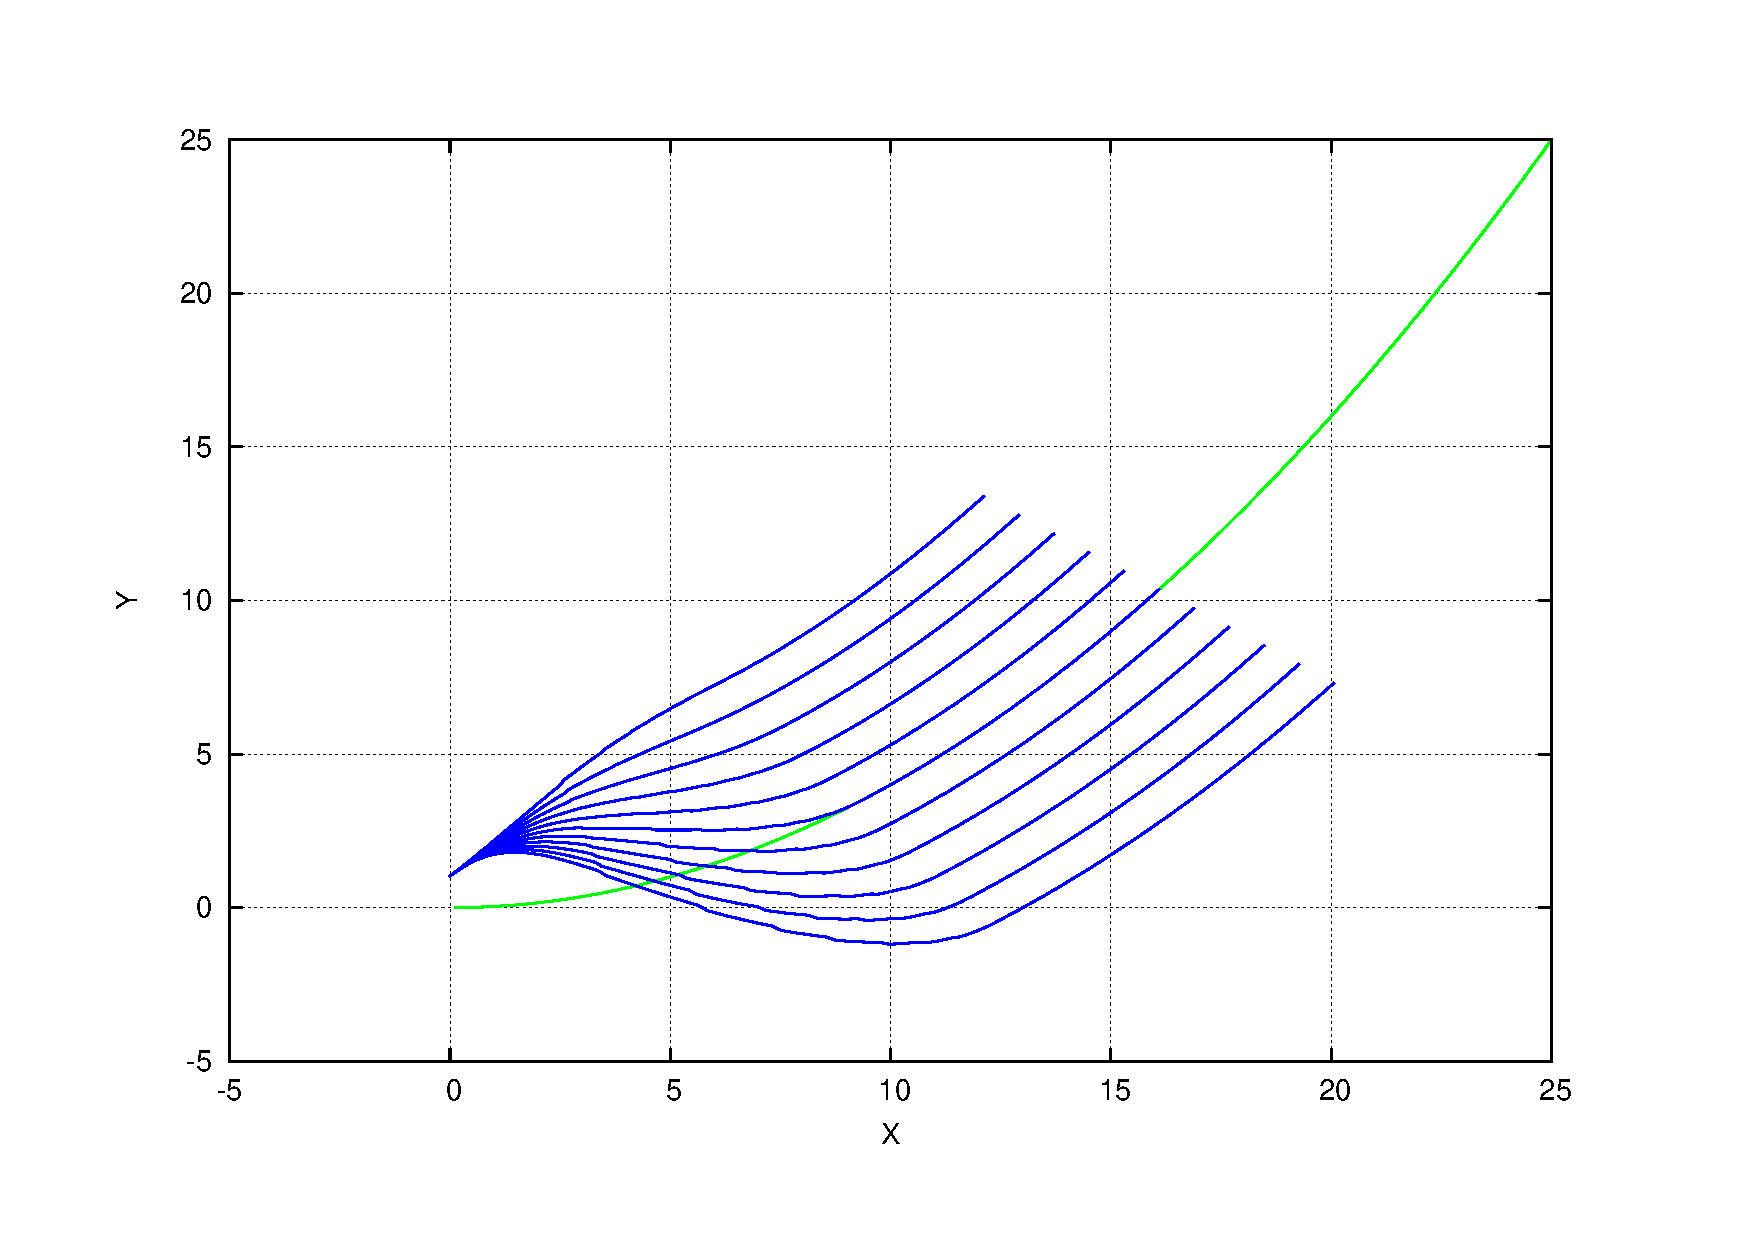
\includegraphics[width=\textwidth, trim=50 40 80 60,clip]{cartesian45}
    \caption{Curvilinear space.}
    \label{fig:cp07_cartesian45}
    \end{subfigure}
\end{tabular}
\caption{Example in which the vehicle is rotated with respect to the path.}\label{fig:cp07_frenet45}
\end{figure}

Now we have the paths in the euclidean distance, we can evaluate which is the maximal distance they can reach individually if obstacles are considered. To do that, we iterate over the points in the trajectory, and check the cost associated to each cell $c_{ij}$ containing the point. If this cost is over the value associated to the threshold $\tau_{circumscribed}$, the path is truncated at this point, as shown in figure \ref{fig:cp07_path_truncation}. The points iterated before reaching this cost will be kept, but it is unlikely that this will be the winner path, as the occlusion cost (see section \todoref{XXX}) will be maximal, and the length of the path shorter (see section \todoref{XXXlengthCost}. The reason for that is that, as the car will be traveling in likely crowded areas, we want to keep moving even if we see that at this point each of the paths do not reach the maximal distance horizon. Obviously, in this case the speed is reduced according to the winner path length. Also, if there is a way to reach the horizon in one of the paths, this will be probably the winner one.

\begin{figure}[h!]
\centering
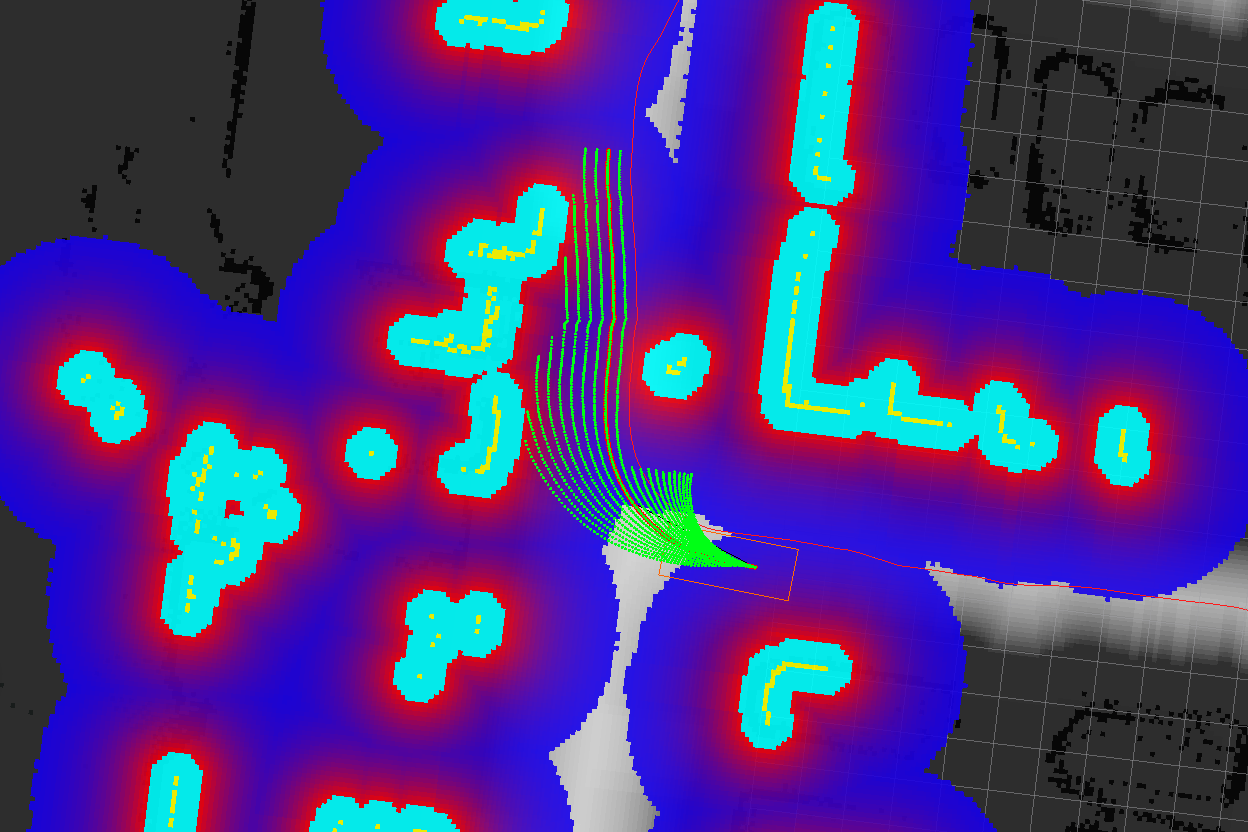
\includegraphics{example15}
\caption{Paths truncation example.}\label{fig:cp07_path_truncation}
\end{figure}

\subsection{Selection of the winner path}\label{ch:chapter07_01_04}

The path is selected from among all the other paths based on a cost function which is a linear combination of other cost functions with weighting factors. The cost function evaluate the occlusion, length, distance to the global path, curvature and consistency of the path as follows:

\begin{equation}\label{eq:cp07_cost_function}
J[i] = \omega_o C_o[i] + \omega_l C_l[i] + \omega_d C_d[i] + \omega_{\kappa} C_{\kappa}[i] + \omega_c C_c[i]
\end{equation}

Here, $i$ is the path index, and $C_o$, $C_l$, $C_d$, $C_{\kappa}$ and $C_c$ are the costs of occlusion, length, distance to the global path, curvature and consistency, respectively. Their relatives $\omega_k$, $k \in \{o, l, d, \kappa, c\}$ are the associate weights that allow to decide the influence of each of the costs to the final cost value.

As we will see in the next sections, all those costs are normalized to $1$, and 

\begin{equation}\label{eq:cp07_weights_sum}
\sum_{{i \in \{o, l, d, \kappa, c\}}} w_i= 1
\end{equation}

, so it is easy to determine the proportional influence of each of the weights with respect to the others. Based on this, the value of $J[i]$ should fall inside the interval $[0\dots1]$.

The following costs will be computed for each candidate path independently in the euclidean space.

\paragraph{Occlusion}\label{ch:chapter07_01_04_00_01}

The occlusion cost is related to the safety of the path. This cost tries to estimate the goodness of a path, being the bests paths those which travel far enough from the obstacles. To do that, we iterate along the path in the way that the footprint of the car is simulated for each position. The cost of occlusion corresponding to the trajectory point $i$, $C_{o,i}$, will be the maximal cost of each of the cells $c_{ij} \in \mathcal{C}$ under the footprint of the car at that position. Based on this, the cost of occlusion will be

\begin{equation}\label{eq:cp07_occlusion_cost}
C_o = {{max\{c_i\}} \over 255}, ~~~~~~ i=1 \dots L
\end{equation}

In this expression, $L$ is the length of the current path. $max\{c_i\}$ is the maximal value of all the costs, each associated to a point in the path. The maximal value of each cost, as we saw before, is $255$. This is the reason for which it is divided by this value, so the values are normalized to $1$.

\paragraph{Length}\label{ch:chapter07_01_04_00_02}

This costs represents the length of the current path. At the same time we iterate over the points in that path for other costs, we accumulate the distance between points, so we know the real distance traveled in euclidean coordinates. The longer a path is, the better, as it means the paths is able to go further. The expression that calculates this cost is:

\begin{equation}\label{eq:cp07_length_cost}
C_l = 1- {{\sum\limits_{i=1}^{L}\|p_i - p_{i - 1}\|} \over {q_{f_{max}} + s_f}}
\end{equation}

Here, $p_i$ is a certain point inside the current path. $q_{f_{max}}$ is the maximal value a $q_f$ can have for a certain path. Lengths are normalized to a value a path could never go beyond in any situation. In our case, we decided that the sum of the maximal expected offset for $s$ and for $q$ will be good enough, as it is safe (lengths will never trespass this value, but it is not too big so paths can be discriminated easily).

As the longer a path is, the better, we subtract it to 1, in order to make it comparable to the rest of costs.

\paragraph{Distance to the global path}\label{ch:chapter07_01_04_00_03}

In our implementation, we included information about the average lateral offset respect to the global path. This information is not considered in the implementation of \cite{chu2012local}. We consider that it is important as we could want to come back to the global path once an occasional obstacle is avoided. In their implementation this possibility is not considered, so the vehicle can remain following a path parallel to the global plan.

This cost is computed as follows:

\begin{equation}\label{eq:cp07_lateral_cost}
C_d = {{\sum\limits_{i=1}^{L}\|p_i - nearest(p_i, g)\|} \over {L \cdot q_{f_{max}}}}
\end{equation}

, where $nearest(p, g)$ is the nearest point in the global path $g$ to the point $p$. This cost is normalized with respect to the maximal expected offset, $q_{f_{max}}$.

\paragraph{Curvature}\label{ch:chapter07_01_04_00_04}

This costs is an attempt to give priority to those paths which are smoother than those with changes in the angle. Let $p_(x_i, y_i), ~ i=1\cdots L$, be a point in the path. Then, 

\begin{equation}\label{eq:cp07_curvature_cost}
C_{\kappa} = max \left \{ {{x_i' \cdot y_i'' - x_i'' \cdot y_i'} \over {(x_i' + y_i')^{3/2}}} \right \}, ~~~~~~ i=1 \dots L
\end{equation}

\paragraph{Consistency}\label{ch:chapter07_01_04_00_05}

This cost tries to keep using a winner path between iterations. Once the vehicle starts a maneuver, it does not change its behavior in the next iteration.

This is done through the following expression:

\begin{equation}\label{eq:cp07_consistency_cost}
C_c = {1 \over {s_2 - s_1}} \int \limits_{s_1}^{s_2} l_i ~ ds
\end{equation}

This equation is better explained if we look at figure \ref{fig:cp07_consistency_cost}. There, the lateral cost $l_i(s)$ is the distance between the current and the previous winner path at a same longitudinal position $s$; $s_1$ and $s_2$ are the first and last positions over $s$ for which there are points in common for both trajectories.

\begin{figure}[h!]
  \centering
  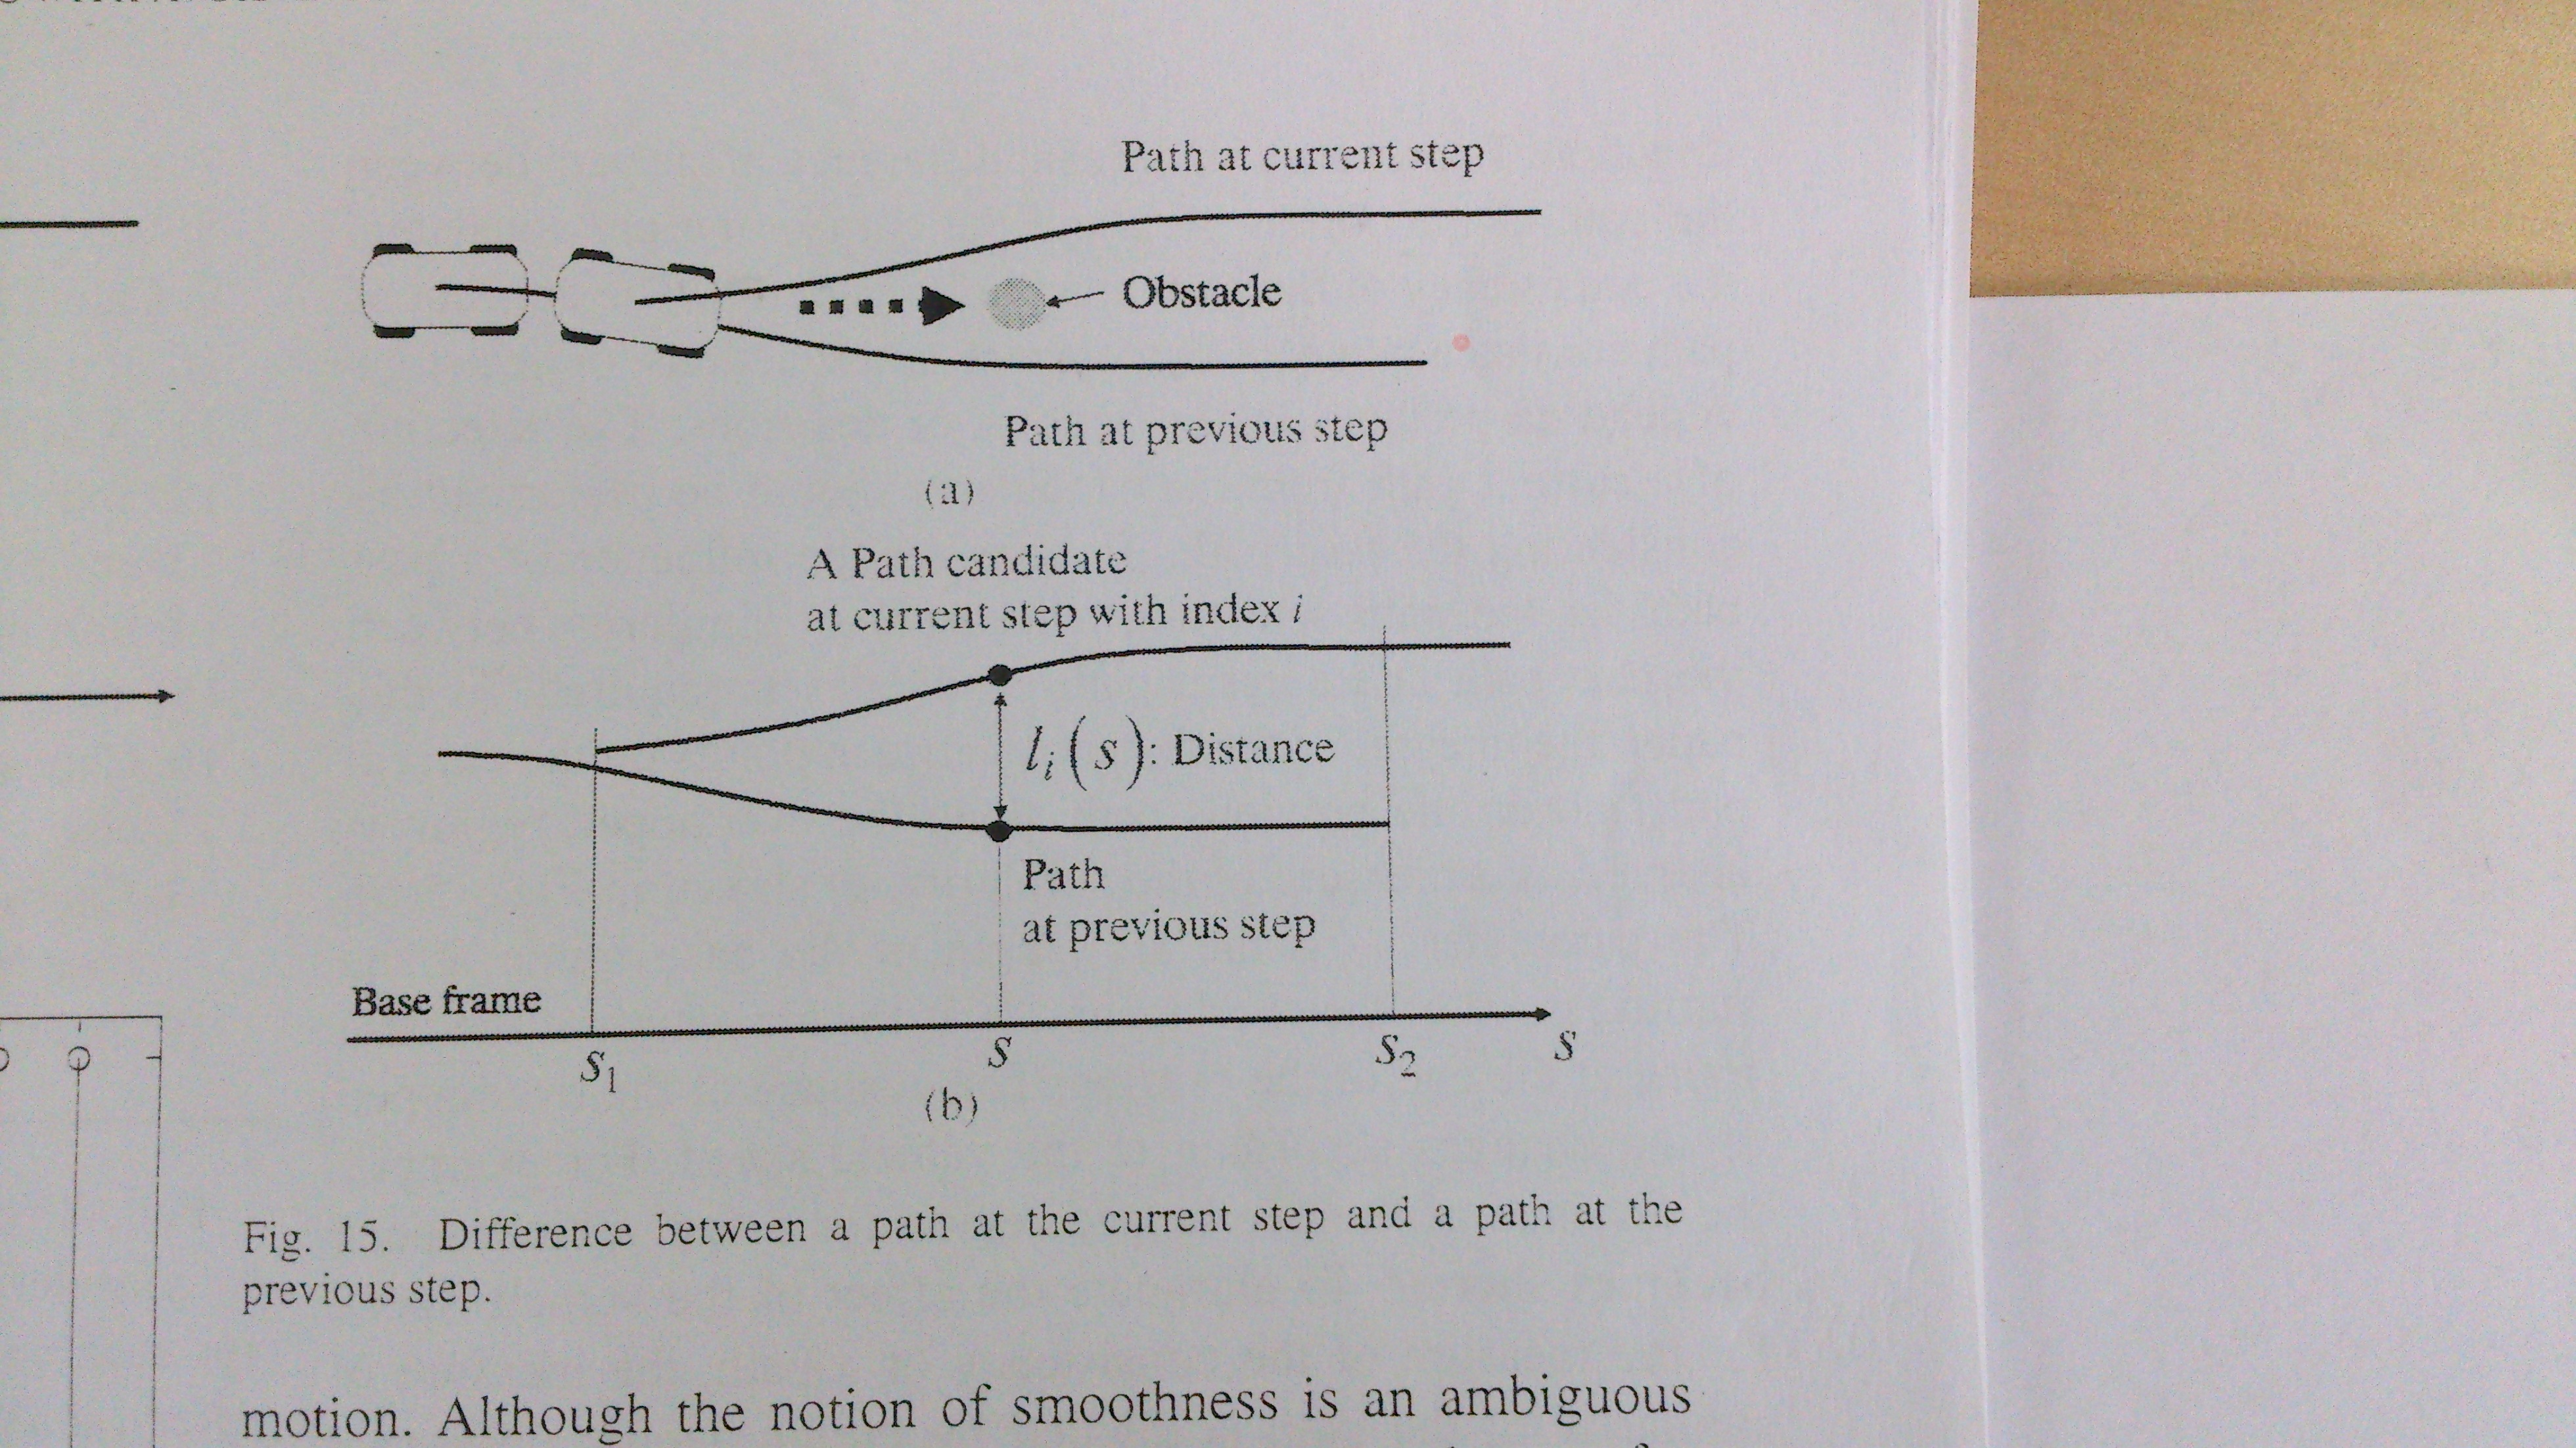
\includegraphics{consistency_cost}
  \caption{Representation of the way in which the consistency cost is computed.}\label{fig:cp07_consistency_cost}
\end{figure}

\subsubsection{Selection of the winner path}\label{ch:chapter07_01_04_01}

With all the costs computed, we just apply the expression described in equation \ref{eq:cp07_cost_function}. Those paths for which it is impossible to advance due to the presence of a nearby obstacle or due to the fact that the car is bad oriented to the global path (which means that no valid paths can be generated in this situation), the cost will be negative (invalid path).

From among all possible values, we select that with the smallest cost, which will be the winner path $W$. If all paths are invalid, that means that the car cannot advance. If the reason is the presence of a nearby obstacle, the vehicle waits until the way is clearer. If this never happens, it generates a new global plan.

In case that the vehicle is bad oriented to the global plan, the recovery behavior process is started.

\subsubsection{Recovery behavior}\label{ch:chapter07_01_04_02}

When the lateral offset of a path is bigger than the radius of curvature of base frame, paths can not be generated using the approach described before. Because of that, we propose to compute the paths in a different way, so the vehicle can advance towards the global plan until this restriction is satisfied. The way in which we do that is through the use of a model of the behavior of the vehicle, which is the same as that used in \todoref{XXX-espelosin}.

Four paths are evolved in a parameterized time $t$, considering a low speed. Two of these paths are generated considering a positive speed (forward movement) and the top left and top right steering position, and the other two are generated for the case of a negative speed. All these four paths are weighted following the same process as in \ref{ch:chapter07_01_04}, and the winner is selected, so the speed and steering commands will be those used to evolve the winner path.

\subsection{Computation of the vehicle commands}\label{ch:chapter07_01_03}

When using this method for path generation, the computation of the speed and steering commands is not straightforward. We have a path that departs from the current position of the vehicle. However, we still have to think how to follow it. The way in which this is done is taking advantage of the bike dynamics model.

This model is represented in figure \ref{fig:cp07_vehicle_commands}.

\begin{figure}[h!]
  \centering
  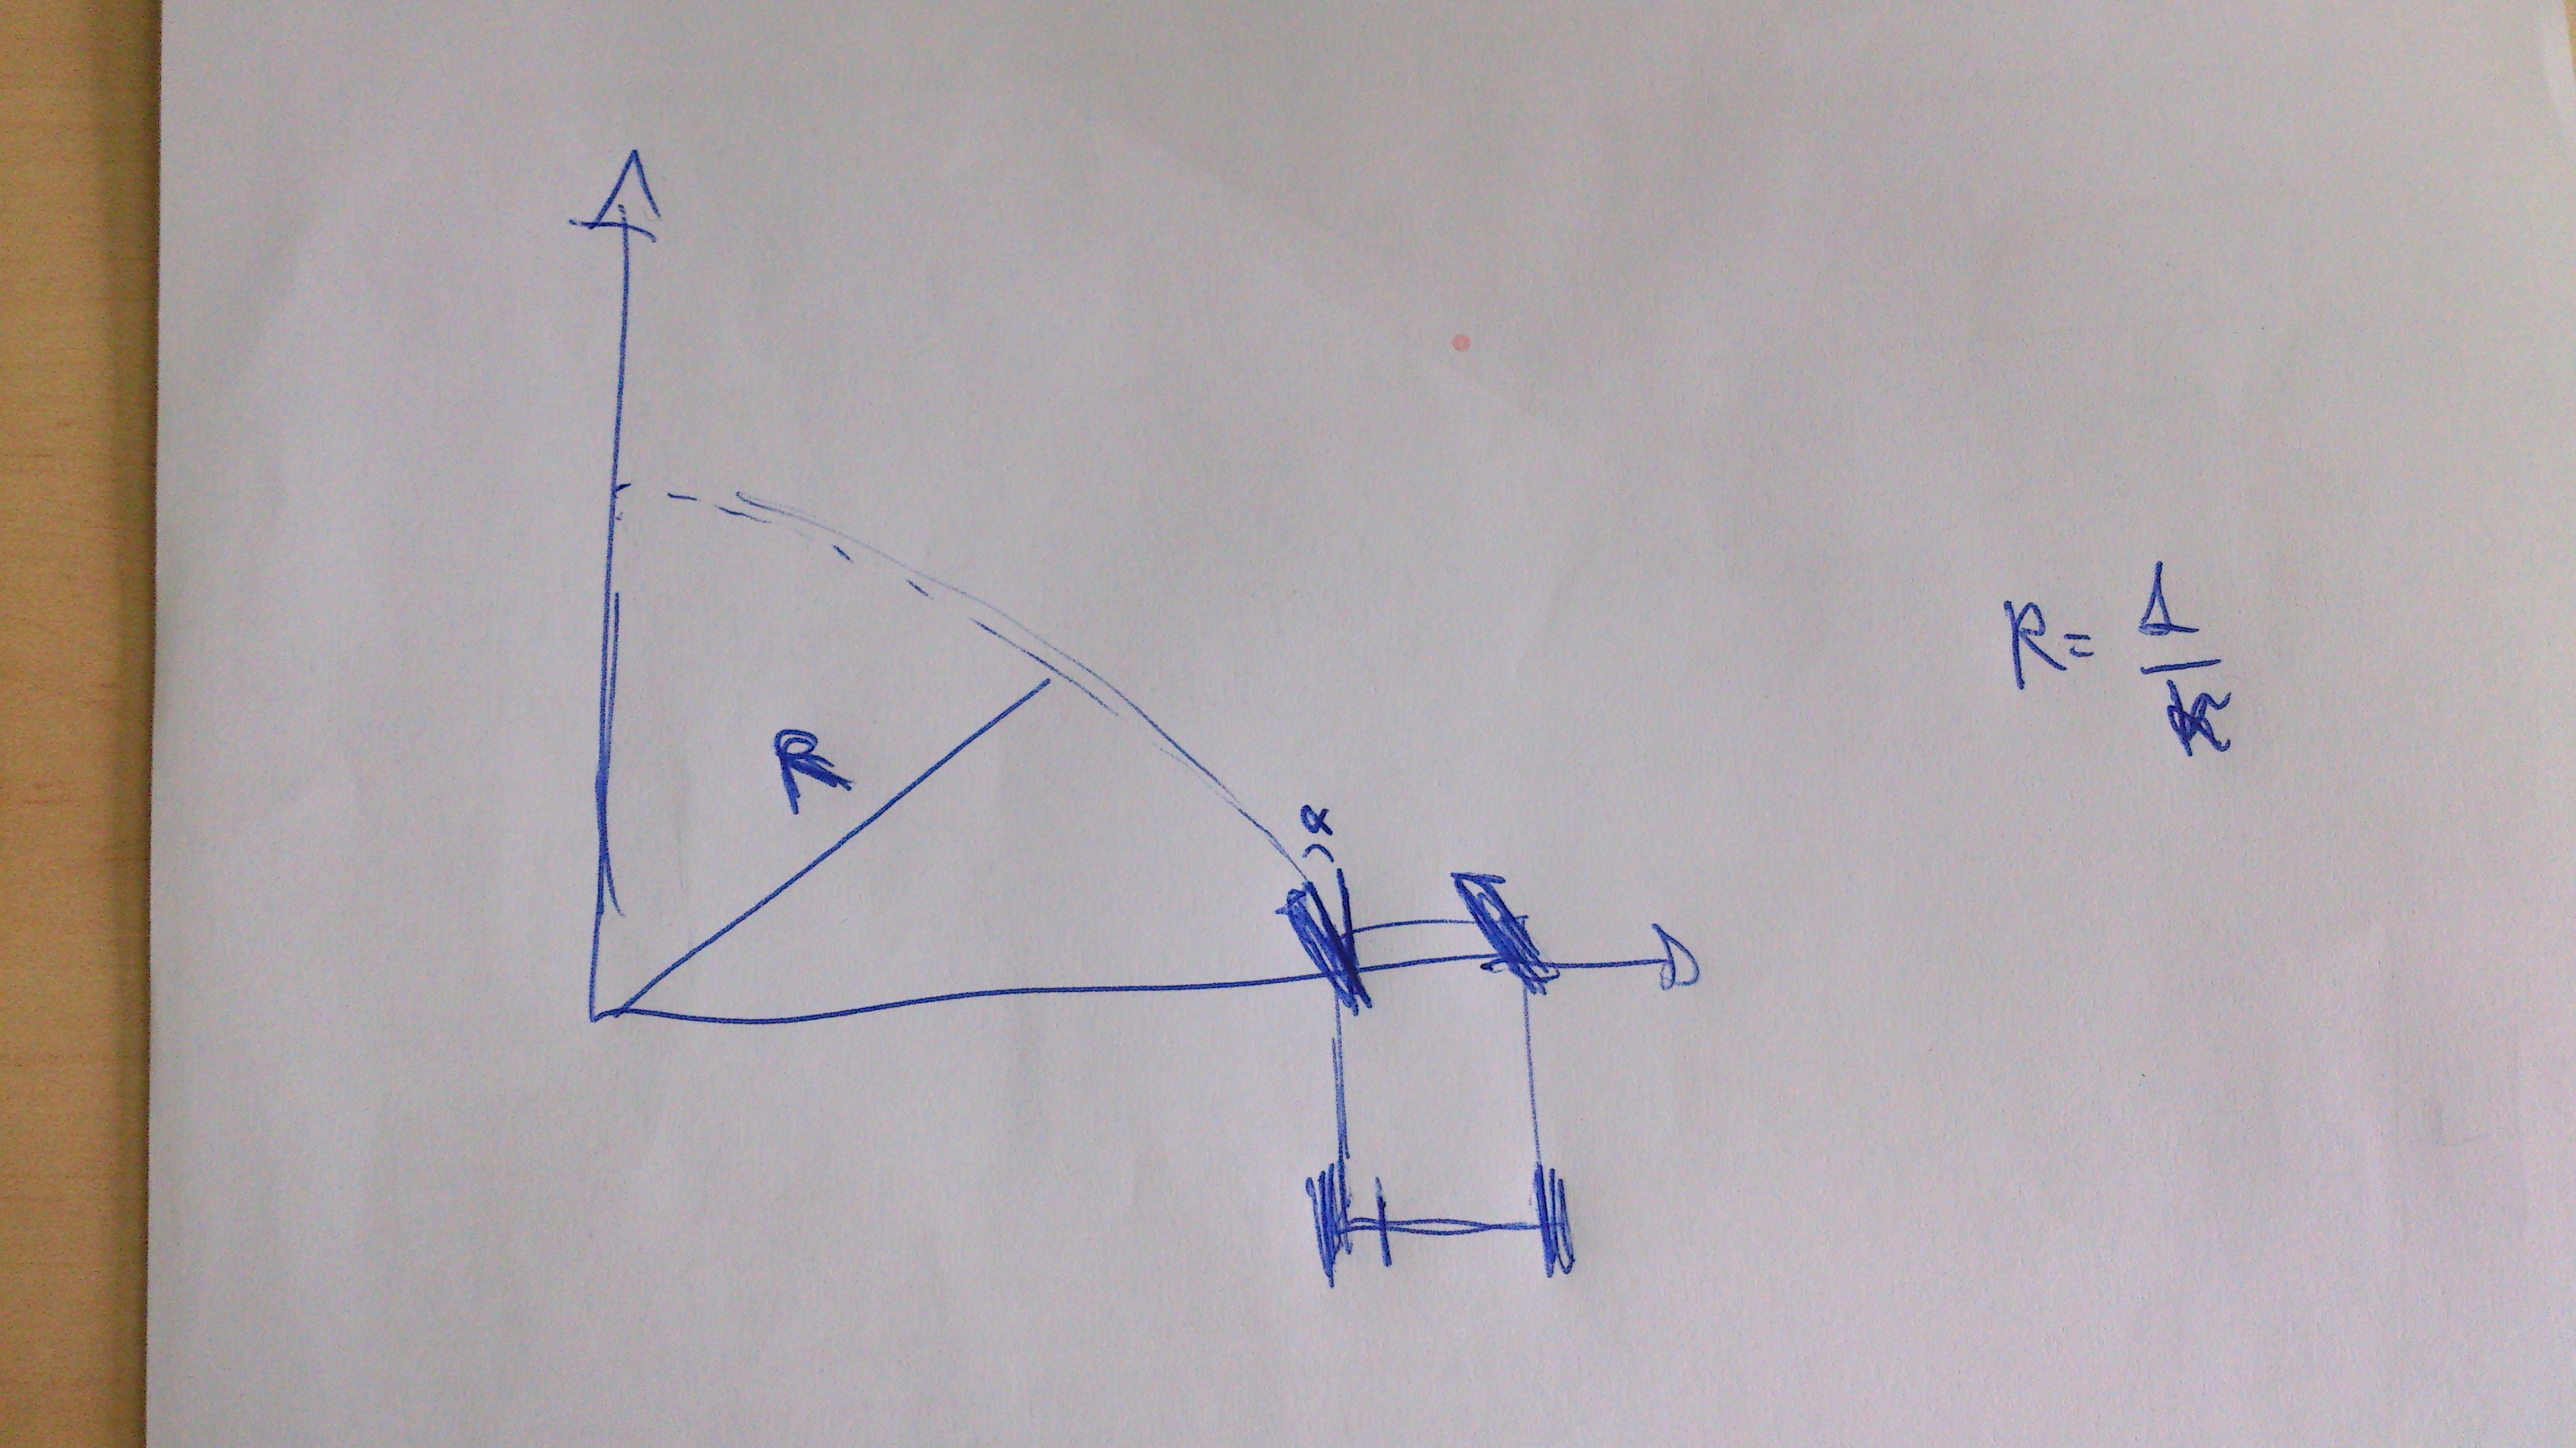
\includegraphics{vehicle_commands}
  \caption{Representation of the model used to recover the steering angle and the speed from a path.}\label{fig:cp07_vehicle_commands}
\end{figure}

As $R = 1 / \kappa$, we just need to compute the curvature for the first $\rho_{steering}$\,m of the winner path. This value will be the steering angle at current time $t$, $\alpha_{t}$, of the vehicle. From this value, we get the speed which is obtained as a linear function of the required steering change.

\begin{equation}\label{eq:cp07_speed_computation}
\dot{v} = \rho_{speed} \cdot v_{max} \cdot | \alpha_{t} - \alpha_{t - 1}|
\end{equation}

, where $\alpha_{t - 1}$ is the steering angle in the last iteration. $\rho_{speed}$ is a constant that allows modifying the influence of the steering increment into the final speed regarding to the maximal speed $v_{max}$.

\section{Summary}\label{ch:chapter07_03}

In this chapter, we have seen a method able to efficiently follow a given trajectory while avoiding the potential obstacles in the way. The use of a curvilinear coordinate system for the generation of a set of candidate trajectories simplifies the calculations while allows creating soft paths that makes the vehicle to converge to the followed track as smooth as possible. Also, these paths are generated with different lateral offsets regarding to the global plan, so we are able to avoid an obstacle even if it is in the middle of the path. Finally, as speed is out the model used for the generation of the tracks, it is reduced to the computation of a set of parameters that define a third order polynomial. Speed and steering angle is then computed based on the shape of the winner path, which is chosen based on a cost function.

As future work, we can study the inclusion of new costs or long-term control strategies, as those used in \cite{werling2010optimal}. Also, the computation of the steering angle based on the winner path is quite rudimentary. We propose as future work the use of a \ac{PID} controller or even a predictive one, as that explained in \todocite{XXX-espelosin}.

In the next chapter, we will see the results obtained for all the methods described before, and how they can be joined together in order to reach the goal initially proposed for this thesis.


